\documentclass[pdf]{beamer}
\mode<presentation>{} 

\usepackage{tabularx}
\usepackage{hyperref}
\usepackage{pgf}
\usepackage{tikz}
\usetikzlibrary{trees}
\usetikzlibrary{arrows,automata}
\usetikzlibrary{automata,positioning}
\usetikzlibrary{shapes}
\usepackage{tikz-qtree,tikz-qtree-compat}
\usepackage{mathtools,enumerate,amssymb}
\usepackage[utf8]{inputenc}
\usepackage[T1]{fontenc}
\usepackage{wrapfig}
\usepackage{setspace}
\usepackage{bbding}
\usepackage{adjustbox}
\usepackage[euler]{textgreek}
\usepackage{multirow}
\usepackage{url}



\definecolor{ballblue}{rgb}{0.13, 0.67, 0.8}
\newenvironment{cirenv}{\only{\setbeamertemplate{items}[circle]}}{}



\title{Flex \& Bison}
\subtitle{Limbaje formale şi translatoare (Compilatoare)}
\AtBeginSection[]{}



\setbeamertemplate{sidebar right}{}
\setbeamertemplate{footline}{%
\hfill\usebeamertemplate***{navigation symbols}
\hspace{1cm}\insertframenumber{}/\inserttotalframenumber}



\begin{document}



\begin{frame}
	\titlepage
	
\begin{flushright}
Mihai-Lica Pura\\
\end{flushright}

\end{frame}


\begin{frame}{Cuprins}
\begin{itemize}
\item
flex (lex)

\item
bison (yacc)

\end{itemize}
\end{frame}



\begin{frame}{lex/flex - Cuprins}
\begin{itemize}
\item
Structura fisierului de intrare

\item
Funcţionarea lex/flex

\item
lex/flex libl

\item
Analiza lexicala contextuala

\item
Depanarea

\end{itemize}
\end{frame}



\begin{frame}{lex/flex}
\begin{itemize}
\item
este un generator de analizoare lexicale în limbajul C
	
	\begin{itemize}
	\item
	\textbf{flex  tokdef.l  $\rightarrow$  lex.yy.c}
	\end{itemize}
	
\item
\textbf{tokedef.l} - fișier de intrare pentru flex

\begin{itemize}
\item
definește \textit{sintaxa atomilor lexicali} ai limbajului sursă (cu ajutorul \textit{expresiilor regulare})
\newline

\item
definește \textit{acțiunile} semantice asociate fiecărei clase de atomi astfel definită
\newline

\item
definitia + actiunea asociata = regula
\newline

\item
în mod obișnuit o actiune se încheie cu returnarea tipului de atom lexical identificat, pentru a putea fi folosit în continuare de catre analizorul sintactic
\end{itemize}

\end{itemize}
\end{frame}



\begin{frame}{lex/flex}
\begin{itemize}
\item
\textbf{lex.yy.c} - fișierul generat de flex pe baza celui de intrare

\begin{itemize}
\item
reprezintă codul sursă al analizorului lexical definit
\newline

\item
contine codul functiei yylex() 
\end{itemize}

\end{itemize}
\end{frame}



\begin{frame}{Fisierul de intrare lex/flex}
\begin{itemize}
\item
Structura fisierului de intrare pentru lex/flex (fisierul .l) este:
 \\~\\
    \color{red}{\%\{ } \\
    \color{red}{define and include directives of cpp} \\
    \color{red}{ \%\} } \\
    \color{red}{definitions} \\~\\
    \color{black}{\%\%} \\~\\
    \color{green}{rules} \\~\\
    \color{black}{\%\%} \\~\\
    \color{blue}{user defined routines}

\end{itemize}
\end{frame}



\begin{frame}{Ex1 din arhiva}
\begin{itemize}
\item[]
\%\{ \\
int charcount=0, linecount=0; \\
\item[]
\%\} \\
\item[]
\%\%
\item[]
. charcount++;
\item[]
\textbackslash n \{lineout++; charcount++;\}
\item[]
\%\%
\item[]
int main()
\item[]
\{
\item[]
yylex(); // End-of-file Ctrl+D
\item[]
printf("There were \%d characters in \%d lines \textbackslash n", charcount, linecount);
\item[]
return 0;
\item[]
\}
\end{itemize}
\end{frame}



\begin{frame}{Fisierul de intrare lex/flex}
\begin{itemize}
\item
codul dintre \% \{ si \% \} este inclus ca atare la începutul fisierului sursa generat

\item
regulile sunt formate din definitiile atomului lexical (expresii regulare) si actiuni corespunzatoare

\item
cele doua componente ale unei reguli sunt despartite printr-un spatiu

\item
la scrierea regulilor este obligatoriu sa se înceapa de pe prima coloana a fiecarei linii

\item
actiunea asociata unei definitii a unui atom lexical se scrie în limbajul de programare C. Daca ea este formata din mai multe instructiuni, acestea trebuie scrise între paranteze acolade.

\end{itemize}
\end{frame}



\begin{frame}{Fisierul de intrare lex/flex}
\begin{itemize}
\item
"user defined routines" poate contine definitii de functii

\item
componenta de baza este functia \textit{main()} care contine apelul functiei \textit{yylex()}, functie care reprezinta de fapt analizorul lexical generat

\item
daca aceasta parte este goala, lex/flex va adauga în mod automat o functie \textit{main} implicita, de forma:

\begin{itemize}
	\item[]
     	\color{red}{int main(int argc, char *argv[])}]

        \item[]
        \color{black}\{

    	 \begin{itemize}
      		\item[]
        	 yylex();


         \item[]
          return 0;
              \end{itemize}


\item[]
\color{black}{\}}
     \end{itemize}
\end{itemize}
\end{frame}



\begin{frame}{Utilizarea lex/flex}
	\begin{itemize}
	\item
	1. Scrierea fisierului de intrare pentru lex/flex 
	
	(e.g. tokdef.l)
	\item
	2. Generarea fisierului sursa a analizorului lexical
	
	(lex.yy.c)
	
		\begin{itemize}
		\item
		\textbf{lex tokdef.l} \color{red} { SAU}
		\item
		\textbf{flex tokdef.l}
		\end{itemize}

	\item		
	3. Compilarea fisierului sursa a analizorului lexical si generarea executabilului

		\begin{itemize}
		\item
		\textbf{cc lex.yy.c -o alex -ll} \color{red} { SAU}
		\item
		\textbf{cc lex.yy.c -o alex -lfl}
		\end{itemize}
	
	\item	
	4. Lansarea in executie
		\begin{itemize}
		\item
		\color{red} {\textbf{./alex}}
		\end{itemize}
	\end{itemize}
\end{frame}



\begin{frame}{Ex2 din arhiva}
\begin{itemize}

\item[]
\%\{ \\
\color{red}{\#include<iostream>} \\
using namespace std;
\color{black}
\item[]
\%\} \\
\item[]
\%\%
\item[]
. \{ \color{red}{cout}\color{black} <<"CAR";\}
\item[]
\textbackslash n \{char*s = \color{red}{new }\color{black} char[4]; \} \\
\item[]
\%\%
\item[]
int main()
\item[]
\{
\item[]
\color{red}{cout}\color{black} \{<<"Incepe";
\item[]
yylex()
\item[]
\color{red}{cout}\color{black} \{<<"Gata";

return 0;
\item[]
\}

\end{itemize}
\end{frame}



\begin{frame}{Utilizarea lex/flex cu cod C++}
\begin{itemize}
\item
1. Scrierea fisierului de intrare pentru lex/flex

(e.g. tokdef.l)

\item
2. Generarea fisierului sursa a analizorului lexical

(lex.yy.c)

\begin{itemize}
\item
\textbf{lex tokdef.l}  \color{red}{  SAU}\color{black}
\item
\textbf{flex.tokdef.l}
\end{itemize}

\item
3. Compilarea fisierului sursa a analizorului lexical si generarea executabilului

\begin{itemize}
\item
\textbf{\color{red} {g++ }\color{black} lex.yy.c -o alex -ll} \color{red} {  SAU}\color{black}
\item
\textbf{\color{red} {g++ }\color{black} lex.yy.c -o alex -lfl}
\end{itemize}

\item
4. Lansarea in executie

\begin{itemize}
\item
\textbf{./alex}
\end{itemize}
\end{itemize}
\end{frame}



\begin{frame}{Functionarea lex/flex}
\begin{itemize}
\item
Expresiile regulate sunt translatate de catre lex/flex într-un program care implementează modul de lucru al unui automat finit determinist.
\newline

\item
Pe baza starii curente si a valorii urmatorului caracter de la intrare, se determina noua stare prin indexarea într-o tabela a starilor generata de catre program.

\end{itemize}
\end{frame}



\begin{frame}{Exemplu de functionare lex/flex}

letter(letter|digit)*   \\~\\

\begin{figure}
\centering
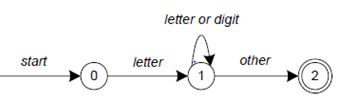
\includegraphics[scale=0.7]{compil4.PNG}\par
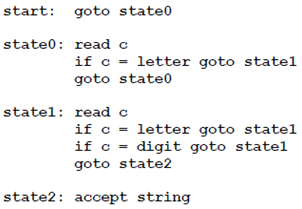
\includegraphics[scale=0.7]{compil5.PNG}\par
\end{figure}

\end{frame}



\begin{frame}{Arhitectura functiei \textit{yylex()}}
int yylex() \\
\{... \\
new\_symbol:\\
switch (c = getchar();)\{\\
case 'a': ... case 'Z': return identifierOrKeyword();\\
case '0': ... case '9': return number();\\
case '(': ... case ')': return specSymbol();\\
case '\textbackslash': return characterOrString();\\
case EOF: return YYEOF;\\
default: error(INVALID\_TOKEN); goto new\_symbol;\\
\}

\end{frame}



\begin{frame}{Sectiunea definitiilor}
\begin{itemize}
\item
1. Cod C - Codul dintre \%\{ si \%\} va fi copiat ca atare la începutul fisierului lex.yy.c. 

\begin{itemize}
\item
directive catre preprocesor (include, definitii s.a.)
\item
definitii de variabile
\item
prototipurile functiilor care vor fi definite în a treia sectiune
\item
ș.a.
\end{itemize}

\item
2. Definitii de aliasuri pentru expresiile regulare – Definitiile elementelor de limbaj care vor fi folosite în regulile din a doua sectiune

\begin{itemize}
\item
letter [a-zA-Z]
\item
digit [0-9]
\item
punct [,:;!?]
\item
nonblank [\^{}  \textbackslash t]
\end{itemize}

\end{itemize}
\end{frame}



\begin{frame}{Sectiunea definitiilor}
\begin{itemize}
\item
3. Definitii de stari - Atunci când o regula depinde de context, se pot defini stari care sa permita identificarea corespunzatoare a atomilor lexicali:

\begin{itemize}
    \item 
    \%s NUMESTARE
\end{itemize}

Exista o stare predefinita si anume starea INITIAL.

\end{itemize}
\end{frame}



\begin{frame}{Sectiunea regulilor}
\begin{itemize}
\item
Contine o serie de perechi definitie-actiune pentru câte o clasa de atomi lexicali

\item 
Definitiile claselor de atomi lexicali sunt expresii regulare scrise si pe baza aliasurilor definite în prima secțiune

\item
Actiunile asociate sunt o instructiune C sau mai multe instructiuni C între paranteze acolade.

\item
Între definitie si actiunea asociata trebuie sa fie cel putin un spatiu (unul sau mai multe spații, unul sau mai multe taburi, dar nu poate fi sfârsitul de linie)

\item 
Adica actiunea asociata unei definitii este obligatoriu sa înceapa de pe aceeasi linie cu aceasta.

\end{itemize}
\end{frame}



\begin{frame}{Sectiunea regulilor}
\begin{itemize}
\item
Scrierea unei reguli trebuie sa înceapa de pe prima coloana a liniei.

\item
Orice text din sectiunea de reguli care nu începe de pe prima coloana a unei linii este copiat ca atare în fisierul sursa generat lex.yy.c.

\item
Daca mai multe definitii se potrivesc textului de intrare, se va lua acea definitie care potriveste textul cel mai lung.

\item 
Daca mai multe definitii potrivesc un text de aceeasi lungime, va fi luata prima în ordinea în care au fost scrise în sectiunea de reguli.

\end{itemize}
\end{frame}



\begin{frame}{Sectiunea regulilor}
\begin{itemize}
\item
. Match any character except newlines.

\item
\textbackslash n A newline character.

\item
\textbackslash t A tab character.

\item
\^{} The beginning of the line.

\item
\$ The end of the line.

\item
\textless expr>* Zero or more occurrences of the expression.

\item
\textless expr>+ One or more occurrences of the expression.

\end{itemize}
\end{frame}



\begin{frame}{Sectiunea regulilor}
\begin{itemize}
\item
\textless expr>? Zero or one occurrences of the expression.

\item
(\textless expr1>|\textless expr2>) One expression or another.

\item
\,[\textless set>] A set of characters or ranges, such as [a-zA-Z].

\item
\,[\^{} \textless set>] The complement of the set, for instance [\^{} \textbackslash t].

\item
"a+b" Liberal "a+b"; C escapes still work!

\item
\textless expr> \{n \} n occurrences of the expression.

\item
\textless expr> \{n, m \} n, n+1, n+2, ... , m occurrences of the expression.
\end{itemize}
\end{frame}



\begin{frame}{Sectiunea regulilor}
\begin{itemize}
\item
Expression \hspace{20mm} Matches
\item
abc \hspace{28mm} abc

\item
abc* \hspace{26mm} ab abc abcc abccc ...

\item
abc+ \hspace{25mm} abc abcc abccc ... 

\item
a(bc)?  \hspace{22mm} one of: a, b, c 

\item
\,[abc] \hspace{28mm} one of: a, b, c

\item
\,[a-z] \hspace{28mm} any letter, a-z 

\end{itemize}
\end{frame}



\begin{frame}{Sectiunea regulilor}
\begin{itemize}
\item
\,[a\textbackslash-z] \hspace{26mm} one of: a, -, z

\item
\,[-az] \hspace{28mm} one of: -, a, z

\item
\,[A-Za-z0-9]+ \hspace{14mm} one or more alphanumeric characters

\item
\,[\textbackslash t \textbackslash n]+ \hspace{22mm} whitespace

\item
\,[\^{}ab] \hspace{28mm} anything except: a,b

\item
\,[a\^{}b] \hspace{28mm} one of: a, \^{}, b

\item
\,[a|b] \hspace{30mm} one of: a, | , b

\item
a|b \hspace{32mm} one of: a,b

\item
(abc)\{2,4\} \hspace{17mm} abcabc or abcabcabc \\ 
\hspace{30mm} or abcabcabcabc

\end{itemize}
\end{frame}



\begin{frame}{Sectiunea regulilor}
\begin{itemize}
\item
Daca pentru anumite succesiuni de caractere nu a fost prevazuta nici o regula, atunci acestora li se aplica \textbf{regula implicita lex/flex} si anume: 

\textbf{potrivirea si copierea caracter cu caracter la iesire}

\item
Ex:
\item
Cel mai scurt fisier de definitii pentru (f)lex este:

\begin{itemize}
    \item 
    \%
\end{itemize}
Actiunea: Intrarea este copiata în iesire, caracter cu caracter.
\end{itemize}
\end{frame}



\begin{frame}{lex/flex libl}
\begin{itemize}
\item
\color{red}{char*yytext} \color{black}- succesiunea de caractere din intrare care se potriveste definitiei curente
\newline
\item
\color{red}{int yyleng} \color{black} - lungimea succesiunii de caractere din intrare care se potriveste definitiei curente (în fapt lungimea sirului de caractere din \textit{yytext})
\newline

\end{itemize}
\end{frame}



\begin{frame}{Ex3 din arhiva}
\begin{itemize}
\item[]
\textbf{\%\{}
\item[]
\textbf{int charcount=0, linecount=0, wordcount=0;}
\item[]
\textbf{\%\}}
\item[]
\textbf{letter[\^{} \textbackslash t \textbackslash n]}
\item[]
\%\%
\item[]
\textbf{\{letter\}+ \{wordcount++; charcount+=yyleng;\}}
\item[]
\textbf{. charcount++;}
\item[]
\textbf{\textbackslash n \{linecount++; charcount++;\}}
\item[]
\textbf{\%\%}
\item[]
\textbf{int main()}
\item[]
\textbf{\{}
\item[]
\textbf{yylex(); // End-of-File Ctrl+D }
\item[]
\textbf{printf("There were \%d word with \%d characters in \%d lines \textbackslash n".wordcount,charcount,linecount);}
\item[]
\textbf{return 0;}
\item[]
\textbf{\}}
\end{itemize}
\end{frame}



\begin{frame}{lex/flex libl}
\begin{itemize}
\item
\textbf{\color{red}FILE* yyout \hspace{3mm} outputfile}
\item
\textbf{\color {red} FILE* yyin \hspace{12mm} inputfile}
\item
Functia \textit{yylex()} citeste textul de analizat prin intermediul variabilei \textit{yyin}, si scrie iesirea prin variabila \textit{yyout}
\newline

\item
În mod implicit:
\begin{itemize}
\item
\textbf{ yyin = stdin}, adica standard input (tastatura) (EOF pentru stdin se poate obține prin \textbf{\color{red}{CTRL+D}})
\item
\textbf{yyout = stdout}, adica standard output (consola) 
\item
 
\end{itemize}

\item
în mod implicit analizorul lexical generat va analiza textul introdus de la tastatura si va scrie iesirea în consolă

\end{itemize}
\end{frame}



\begin{frame}{Ex4 din arhiva}
\begin{itemize}
\item[]
\%\{
\item[]
int lineno;
\item[]
\%\}
\item[]
\%\%
\item[]
\^{}(.*)\textbackslash n fprintf(yyout, "\%4d \textbackslash t \%s", ++lineno, yytext);
\item[]
\%\%
\item[]
int main(int argc, char*argv[])\{
\item[]
\color{red}{yyin=fopen(argv[1], "r")};
\item[]
yyout=fopen(argv[2], "w");
\item[]
\color{black}{\textbf{yylex();}}
\item[]
\color{red}{\textbf{fclose(yyin);}}
\item[]
\color{red}{\textbf{fclose(yyout);}}
\item[]
\color{black}{\}}

\end{itemize}
\end{frame}



\begin{frame}{lex/flex libl}
\begin{itemize}
\item
\textbf{\color{red}{int yywrap(void)}}
\item
atunci când \textit{yylex}, citind din \textit{yyin}, ajunge la EOF se apeleaza automat functia \textit{yywrap()}
\newline

\item
\textbf{yywrap()} returneaza 
\begin{itemize}
\item
1 daca nu mai exista intrare de analizat
\item
0 daca mai exista cel puțin o intrare de analizat
\end{itemize}

\item
functia \textbf{yywrap()} împreuna cu \textbf{yyin} si \textbf{yyout} poate fi folosita pentru a analiza consecutiv mai multe fisiere de intrare si respectiv pentru a scrie consecutiv în mai multe fisiere de iesire

\end{itemize}
\end{frame}



\begin{frame}{Ex5 din arhiva}
\begin{itemize}
\item[]
\%\{
\begin{itemize}
    \item[]
    \#include \textless string.h>
    \item[]
    \color{red}{int second\_file=0;}
    \item[]
    char *nume2;
    \item[]
    int lineno;
\end{itemize}
\item[]
\%\}
\item[]
\%\%
\item[]
\^{}(.*) \textbackslash n fprintf(yyout, "\%4d \textbackslash t \% s", ++lineno, yytext);
\item[]
\%\%
\item[]
int main(int argc, char *argv[]) \{
\begin{itemize}
    \item[]
    \color{red}{nume2=(char*)malloc(sizeof(char)*(strlen(argv[2]+1));}
    \item[]
    \color{red}{strcpy(nume2, argv[2]);}
    \item[]
    yyin = fopen(argv[1], "r");
    \item[]
    yyout = fopen(argv[3], "w");
    \item[]
    yylex()
    \item[]
    fclose(yyin);
    \item[]
    fclose(yyout);

\end{itemize}
\item[]
\}

\end{itemize}
\end{frame}



\begin{frame}{Ex5 din arhiva}
\begin{itemize}
\item[]
int yywrap()
\item[]
\{
\begin{itemize}
    \item[]
    if(second\_file ==0)
    \item[]
    \{
    \begin{itemize}
        \item[]
        fclose(yyin);
        \item[]
        \color{red}{yyin=fopen(nume2, "r");}
        \item[]
        \color{black}{second\_file=1;}
        \item[]
        \color{red}{return 0;}
    \end{itemize}
    \item[]
    \}
\end{itemize}
\item[]
else
\begin{itemize}
    \item[]
    \color{red}{return 1;}
\end{itemize}
\item[]
\}

\end{itemize}
\end{frame}



\begin{frame}{lex/flex libl}
\begin{itemize}
\item
\color{red}{int yymore(void)} \color{black}{- append the next token to \textit{yytext}}
\item
\color{red}{int yyles(int n)} \color{black}{- truncate the current token to n characters}
\item
\color{red}{int input(void)} \color{black}{- extract the next symbol from input}
\item
\color{red}{int unput(int c)} \color{black}{- return the symbol c back to the input}
\item
\color{red}{int yylineno} \color{black}{- current line number}

\end{itemize}
\end{frame}



\begin{frame}{Depanare lex/flex}
\begin{itemize}
\item
Codul generat de catre lex/flex în lex.yy.c contine si instructiunii de depanare.

\item
Acestea pot fi activate prin specificarea parametrului \textbf{-d} la etapa de generare a fisierului sursa a analizorului lexical.
\newline

\item
Adica:
\item
\begin{itemize}
    \item[]
    lex -d tokdef.l
    \item[]
    flex -d tokdef.l
\end{itemize}

\end{itemize}
\end{frame}



\begin{frame}{Dependenta de context}
\begin{itemize}
\item
Daca aplicarea unei reguli depinde de context, atunci analizorul lexical generat trebuie sa fie în masura sa faca o analiza în functie de context.
\newline

\item 
Prin context se înțelege locatia în cadrul codului sursa care trebuie analizat a succesiunii de caractere la care se refera regula respectiva.
\newline

\item
Pentru a trata astfel de operatii, lex/flex permite utilizarea:
\begin{itemize}
\item
\textbf{right state}: aplicarea unei reguli depinde de ceea ce urmeaza dupa succesiunea de caractere respective

\item
\textbf{left state}: aplicarea unei reguli depinde de ceea ce a fost înaintea succesiunii de caractere respective
\end{itemize}
\end{itemize}
\end{frame}



\begin{frame}{Dependenta de context}
Exemplu
\begin{itemize}
\item
Sa se genereze un analizor lexical care sa modifice numele claselor, metodelor si variabilelor conform conventiei Java de denumire: numele claselor încep cu litera mare, iar numele variabilelor si ale metodelor încep cu litera mica.
\newline

\item
atomii lexicali corespunzatori celor trei tipuri de identificatori au aceeasi definitie, si anume:
\begin{itemize}
    \item 
    \,[a-zA-Z][a-zA-Z0-9]*
\end{itemize}

\item
actiunea asociata definitiilor trebuie însa sa fie diferita:

\begin{itemize}
\item
pentru numele de clase trebuie capitalizata prima litera

\item
pentru numele de variabile si de metode, prima litera trebuie sa fie transformata în litera mica
\end{itemize}

\item
\textbf{cum se face diferența?}

\end{itemize}
\end{frame}



\begin{frame}{Left state}

\begin{figure}
\centering
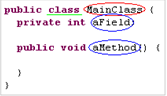
\includegraphics[scale=1.5]{comp.PNG}
\end{figure}


\end{frame}



\begin{frame}{Left state}
\begin{itemize}
\item
Daca gândim problema ca fiind una de dependenta de context de tip stânga, atunci:

\begin{itemize}
\item
daca \textbf{înainte} de identificator a fost cuvântul cheie \textbf{class} urmat de cel putin un spatiu, atunci identificatorul este un nume de clasa si trebuie capitalizat primul lui caracter
\newline

\item
daca înainte de identificator a fost orice altceva, atunci el este un nume de variabila sau de metoda si primul sau caracter trebuie transformat în litera mica
\end{itemize}

\end{itemize}
\end{frame}



\begin{frame}{Impementarea left state}
\begin{itemize}
\item
regula este prefixata cu numele unei stari, sub forma:
\\
\textbf{<NUME\_STARE> definitie\_atom\_lexical actiune}
\newline

\item
regula va fi evaluata numai daca analizorul lexical se afla în starea <NUME\_STARE> respectivă
\newline

\item
schimbarea starii curente a analizorului lexical se poate face în partea de actiuni a unei reguli cu ajutorul macroului BEGIN:
\\
\textbf{NUME\_STARE>definitie\_atom\_lexical \{actiuni;\\
\hspace{40mm}BEGIN NUME\_ALTA\_STARE;\}}
\newline

\item
toate starile trebuie definite în sectiunea de definitii a primei parti a fisierului de intrare printr-o instructiune de forma:
\\
\hspace{25mm} \textbf{\%s NUME\_STARE}
\newline

\item
Starea initiala a analizorului este \textbf{INITIAL}

\end{itemize}
\end{frame}



\begin{frame}{Implementare left state}
\begin{figure}
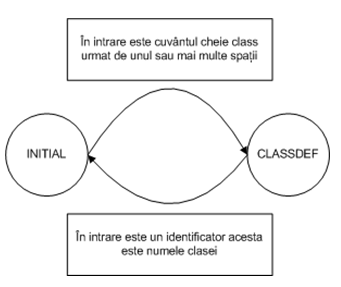
\includegraphics[scale=0.8]{compil3.PNG}
\end{figure}

\end{frame}



\begin{frame}{Ex7 din arhiva}
\begin{itemize}
\item[]
\%\{
\begin{itemize}
    \item[]
    \#include<string.h>
\end{itemize}
\%\}
\item[]
\color{red}{\%s CLASSDEF} \\~\\
\item[]
\color{black} {\%\%} \\~\\

\item[]
\color{red}{<INITIAL>} \color{black} [a-zA-Z][a-zA-Z0-9]*\{yytext[0]=(char)tolower(yytext[0]);\\
fprintf(yyout, "\%s", yytext); \color{black}{\}}

\item[]
\textless INITIAL>"class"[]+\{ ECHO; \color{red}{BEGIN CLASSDEF;} \color{black}{\}}

\item[]
\color{red}{<CLASSDEF>} \color{black} [a-zA-Z][a-zA-Z0-9]*\{yytext[0]=(char)tolower(yytext[0]);\\
fprintf(yyout, "\%s", yytext); \color{red}{BEGIN INITIAL;}
\item[]
\color{black}{\}}
\item[]
.ECHO;
\item[]
\textbackslash n ECHO;
\item[]
\%\%
\end{itemize}
\end{frame}



\begin{frame}{Right state}

\begin{figure}
\centering
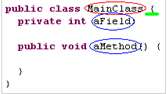
\includegraphics[scale=1.5]{compil2.PNG}
\end{figure}

\end{frame}



\begin{frame}{Right state}
\begin{itemize}
\item
Daca gândim problema ca fiind una de dependenta de context de tip dreapta, atunci:

\begin{itemize}
\item
daca dupa identificator urmeaza cel putin un spatiu si \textbf{apoi} o \textbf{paranteza acolada deschisa}, atunci identificatorul este un nume de clasa si trebuie capitalizat primul lui caracter
\newline

\item
daca dupa identificator urmeaza orice altceva, atunci el este un nume de variabila sau de metoda si primul sau caracter trebuie transformat în litera mica
\end{itemize}

\end{itemize}
\end{frame}



\begin{frame}{Implementarea right state}
\begin{itemize}
\item
specificarea contextului dreapta se face cu ajutorul caracterului \color{red}{/} \color{black}{}

\item
regula respectiva  va avea forma: 

\textbf{definitie\_atom\_lexical/context actiune} \\

\item
succesiunea de caractere care defineste contextul dreapta ramâne în sirul de intrare si va fi analizata ulterior de catre analizorul lexical

\end{itemize}
\end{frame}



\begin{frame}{Ex6 din arhiva}
\%\{\\
\hspace{4mm} \#include<string.h>\\
\%\}\\
\%\%\\
\,[a-zA-Z]\,[a-zA-Z0-9]*/\,[\textbackslash t \textbackslash n]+[\{] \{yytext[0]=(char)toupper(yytext[0]); fprintf(yyout, "\%s", yytext);\}\\
\,[a-zA-Z]\,[a-zA-Z0-9]* yytext[0]=(char)tolower(yytext[0]);fprint(yyout, "\%s", yytext);\}\\
.ECHO;\\
\textbackslash n ECHO;\\
\%\%
\end{frame}



\begin{frame}{Exemplu}
\begin{itemize}
\item
Suppose we want to clean up sloppy spacing and punctuation in typed text. For example in this text: \\~\\

\textit{This \hspace{4mm} text \hspace{2mm} (all of it \hspace{3mm})has occasional lapses , in punctuation(sometimes pretty bad) ,( sometimes not so) . \\~\\
(Ha!) is this: fun? Or what!}
\end{itemize}
\end{frame}



\begin{frame}{Exemplu}
We have
\begin{itemize}
\item
\hspace{6mm} Multiple consecutive blank line: those should be compacted.
\item
\hspace{6mm} Multiple consecutive spaces, also to be compacted.
\item
\hspace{6mm} Space before punctuation and after opening parentheses.
\item
\hspace{6mm} Missing spaces before opening and after closing parentheses.
\item
The last item is a good illustration of where state comes in: a closing paren folloed by punctuation is allowed, but followed by a letter it is an error to be corrected.
\end{itemize}
\end{frame}



\begin{frame}{Ex8 din arhiva}
\begin{itemize}
\item[]
punct [,.;!?]
\item[]
text[a-zA-Z]
\item[]
\%\%
\item[]
"\,)"" "+/ \{punct\} \hspace{5mm} \{printf(")");\}
\item[]
")"/\{text\} \hspace{5mm} \{printf(")");\}
\item[]
\{text\}+" "+/")" \hspace{5mm} \{while(yytext[yyleng-1]=='')yyleng--; ECHO;\}
\item[]
(\{punct\}|\{text\}+)/"(" \hspace{5mm} \{ECHO; printf(" ");\}
\item[]
"("" "+/\{text\} \hspace{5mm} \{while(yytext[yyleng-1]=='')yyleng--; ECHO;\}
\item[]
\{text\}+" "+/\{punct\} \hspace{5mm} \{while(yytext[yyleng-1]=='')yyleng--; ECHO;\}
\item[]
\^{}+ \hspace{5mm} ;
\item[]
" "+ \hspace{5mm} \{printf(" ");\}
\item[]
. \hspace{5mm} \{ECHO;\}
\item[]
\textbackslash n / \textbackslash n \textbackslash n \hspace{5mm} ;
\item[]
\textbackslash n \hspace{5mm} \{ECHO;\}
\end{itemize}
\end{frame}



\begin{frame}{Ex9 din arhiva}
\begin{itemize}
\item[]
punct[,.;:!?]
\item[]
text [a-zA-Z]
\item[]
\%s OPEN
\item[]
\%s CLOSE
\item[]
\%s TEXT
\%s PUNCT \\~\\
\%\%
\end{itemize}
\end{frame}



\begin{frame}{Ex9 din arhiva}
\begin{itemize}
\item[]
" "+ \hspace{40mm} ;
\item[]
\textless  INITIAL>"(" \hspace{5mm} \{ECHO; BEGIN OPEN;\}
\item[]
\textless  TEXT>"(" \hspace{5mm} \{printf(" ") ECHO; BEGIN OPEN;\}
\item[]
\textless  PUNCT>"(" \hspace{5mm} \{printf(" ") ECHO; BEGIN OPEN;\}
\item[]
")" \hspace{5mm} \{ECHO; BEGIN CLOSE;\}
\item[]
\textless INITIAL>\{text\}+ \hspace{5mm} \{ECHO; BEGIN TEXT;\}
\item[]
\textless OPEN>\{text\}+ \hspace{5mm} \{ECHO; BEGIN TEXT;\}
 \item[]
\textless CLOSE>\{text\}+ \hspace{5mm} \{printf(" "); ECHO; BEGIN TEXT;\}
\item[]
\textless TEXT>\{text\}+ \hspace{5mm} \{printf(" "); ECHO; BEGIN TEXT;\}
\item[]
\textless PUNCT>\{text\}+ \hspace{5mm} \{printf(" "); ECHO; BEGIN TEXT;\}
\item[]
\{punct\}+ \hspace{5mm} \{ECHO; BEGIN PUNCT;\}
\item[]
\textbackslash n \hspace{5mm} \{ECHO; BEGIN INITIAL;\}
\item[]
\%\%
\end{itemize}
\end{frame}



\begin{frame}{Cuvinte rezervate}
\begin{itemize}
\item
Daca limbajul pentru care este generat analizorul lexical are un numar mare de cuvinte cheie, atunci este mai eficient sa folosim lex/flex pentru a potrivi identificatorii si sa alegem noi din cod care dintre acestia sunt cuvinte cheie, comparându-i, de exemplu, cu intrarile dintr-o tabela de cuvinte rezervate.
\newline

\item
adica in loc de:
\begin{itemize}
    \item[]
    \textbf{"if" \hspace{35mm} return IF;}
    \item[] 
    \textbf{"then" \hspace{20mm} return THEN;}
    \item[] 
    \textbf{"else" \hspace{24mm} return ELSE;}
    \item[] 
    \textbf{\{letter\}(\{letter\}|\{digit\})* \{ }
    \begin{itemize}
        \item 
        \textbf{yytlval.id=symLookup(yytext);}
        \item
        \textbf{return IDENTIFIER;}
        \item
        \textbf{\}}
    \end{itemize}
\end{itemize}
\end{itemize}
\end{frame}


\begin{frame}{Cuvinte rezervate}
\begin{itemize}
\item
sa se foloseasca: \\~\\
\item[] 
\textbf{\{letter\}(\{letter\}|\{digit\})* \{ }
\begin{itemize}
    \item[] 
    \textbf{int i;}
    \item[]
    \textbf{if((i=resWord(yytext))!=0)}
    \begin{itemize}
        \item[] 
        \textbf{return(i);}
    \end{itemize}
    \item[]
    \textbf{yylval.id=symLookup(yytext);}
    \item[]
    \textbf{return (IDENTIFIER);}
    \item[]
    \textbf{\}}
\end{itemize}

\end{itemize}
\end{frame}



\begin{frame}{Implementarea unui analizor lexical}
\begin{itemize}
\item
Utilizarea lex/flex pentru a implementa un analizor lexical pentru un limbaj de programare:
\newline

\begin{itemize}
    \item 
    - definirea claselor de atomi lexicali
    \item
    - ș.a \\~\\
\end{itemize}
\item
Ex:

\end{itemize}
\end{frame}



\begin{frame}{Limitarile lex/flex}
\begin{itemize}
\item
Cauze: provin din modul în care este implementat - prin automate finite deterministe
\newline
\item
Consecinta: lex/flex are numai stari si tranzitii între stari
\newline
\item
De exemplu, lex/flex nu poate fi utilizat pentru a recunoaste structuri îmbricate, cum ar fi parantezele
\newline
\item
Tratarea structurilor îmbricate cu ajutorul lui (f)lex se poate face numai prin utilizarea unei stive (implementata si gestionata de catre programator).

\end{itemize}
\end{frame}



\begin{frame}{Depanarea codului sursa}
\begin{itemize}
\item[1]
Tinem minte numarul liniei/liniilor din cadrul fisierului \textbf{.l}, de unde dorim sa facem debug (il vom folosi pentru a seta breakpoint-urile)
\newline

De exemplu, pentru a face debug in functia main, pentru fisierul \textbf{ex.l} cu continutul de pe slide-ul urmator, vom tine minte numarul  \textbf{8}.
\end{itemize}
\end{frame}



\begin{frame}{Depanarea codului sursa}
\begin{itemize}
\item[]
\%\{
\item[]
int lineno;
\item[]
\%\}
\item[]
\%\%
\item[]
\^{}(.*)\textbackslash n fprintf(yyout, "\%4d \textbackslash t \%s", ++lineno, yytext);
\item[]
\%\%
\newline
int main(int argc, char*argv[])\{
\item[]
color{red}{yyin=fopen(argv[1], "r"};
\item[]
yyout=fopen(argv[2], "w");
\item[]
\color{black}{\textbf{yylex();}}
\item[]
\color{red}{\textbf{fclose(yyin);}}
\item[]
\color{red}{\textbf{fclose(yyout);}}
\item[]
\color{black}{\}}

\end{itemize}
\end{frame}



\begin{frame}{Depanarea codului sursa}
\begin{itemize}
\item[2]
Folosim lex/flex pentru a genera codul sursa al instrumentului de analiza lexicala, pe baza fisierului ex.l.    \\
\hspace{10mm} \textbf{flex ex.l}
\item[3]
Compilam pentru debug codul sursa obtinut, adaugând optiunea -\textbf{g} pentru a genera un executabi\\
\hspace{10mm} \textbf{gcc lex.yy.c -g -o executabil -lfl}

\end{itemize}
\end{frame}



\begin{frame}{Depanarea codului sursa}
\begin{itemize}
\item[4]
Lansam debuggerul \textbf{gdb} trasmitându-i ca si parametru numele executabilului pe care dorim sa îl depanam
\\
\hspace{10mm} \textbf{gdb executabil}\\
\item[5]
Setam breakpoint-urile folosind comanda  -\textbf{b sau break}, numele fisierului .l si numarul liniei pe care dorim sa setam breakpoint-ul\\
\hspace{10mm} \textbf{b ex.l:8}\\
\item[6]
Repetam pasul al 5-lea pentru fiecare breakpoint pe care dorim sa îl setam

\end{itemize}
\end{frame}



\begin{frame}{Depanarea codului sursa}
\begin{itemize}
\item[7]
Lansam procesul de depanare cu comanda\\
\hspace{10mm} \textbf{run}\\
\item
Daca executabilul asteapta sa primeasca argumente la lansarea în executie (de exemplu numele fisierelor de intrare si de iesire) acestea vor fi furnizate ca si argumente ale comenzii run. De exemplu\\
\hspace{10mm} \textbf{run in.txt out.txt}\\
\item
Daca executabilul lucreaza cu \textit{stdin} si \textit{stdout}, dupa comanda run el va astepta sa introducem textul de analizat.
\end{itemize}
\end{frame}



\begin{frame}{Depanarea codului sursa}
\begin{itemize}
\item[8]
Programul va rula pâna la primul breakpoint întâlnit în executie si apoi se va opri afisând instructiunea de la acel breakpoint
\item
În acel moment se va putea vizualiza valoarea unei variabile (echivalentul unui watch) cu comanda \textbf{p sau print} urmata de numele variabilei a carei valoarea dorim sa o vizualizam\\
\hspace{10mm} \textbf{p yytext}\\
\item[9]
Executia instructiunii curente si oprirea la instructiunea urmatoare se face cu comanda  \textbf{n sau next}\\
\hspace{10mm} \textbf{n}\\

\end{itemize}
\end{frame}



\begin{frame}{Depanarea codului sursa}
\begin{itemize}
\item[10]
Executia programului pâna la urmatorul breakpoint setat se face cu comanda \textbf{c sau continue}\\
\hspace{10mm} \textbf{c}\\
\item[11]
Iesirea din debugger se face cu comanda \textbf{q sau quit} \\~\\
\end{itemize}
\end{frame}



\begin{frame}{Depanarea codului sursa}
Tutoriale gdb
\begin{itemize}
\item
\url{http://www.unknowroad.com/com/rtfm/gdbtut/}

\item
\url{http://www.cs.umd.edu/~srhuang/teaching/cmsc212/gdb-tutorial-handout.pdf}

\item
\url{http://www.cs.cmu.edu/~gilpin/tutorial/}
\end{itemize}
\end{frame}



\begin{frame}{flex - Exercițiu}

\begin{itemize}
\item
Să se implementeze folosind flex un instrument de analiză lexicală care, pentru un fişier de intrare care conţine cod sursă C/C++/C\#, să genereze un fişier de ieşire în care codul este aliniat cu numărul corespunzător de taburi, în funcţie de parantezele acolade.

\item
Să se implementeze folosind flex un instrument de analiză lexicală care, pentru un fişier de intrare care conţine cod sursă C/C++/C\#, să genereze un fişier de ieşire care:
\begin{itemize}
\item
să conţină toate numele variabilelor globale;
\item
să conţină toate numele variabilelor locale pentru fiecare funcţie definită în parte;
\item
să conţină toate comentariile pentru instrucţiunile din fiecare funcţie în parte.
\end{itemize}
\end{itemize}
\end{frame}



\begin{frame}{yacc/bison - Cuprins}
\begin{itemize}
\item
Structura fisierului de intrare

\item
Analiza sintactica

\item
Funcţionarea yacc (bison)

\item
Precedenţa şi asociativitatea operatorilor

\item
Conflicte shift/reduce

\item
Conflicte reduce/reduce

\item
Tratarea erorilor

\item
Depanarea

\item
Transmiterea informatiilor privind locatia atomilor lexicali

\item
Transmiterea valorii semantice a atomilor lexicali

\item
Analiza semantica

\item
Generarea codului pentru limbajul expresiilor aritmetice

\end{itemize}
\end{frame}



\begin{frame}{yacc/bison}
\begin{itemize}
	\item
	“Yet another compiler’s compiler” este un generator de analizoare sintactice, capabile să parseze un şir de atomi lexicali, care, de obicei, este generat cu ajutorul instrumentului lex/flex.

	\item
	Dacă lex/flex are nevoie de definiţiile atomilor lexicali pentru a fi în măsură să îi descopere într-un şir de intrare, yacc/bison are nevoie de definiţia limbajului de analizat, dată printr-o gramatică generatoare.
\end{itemize}
\end{frame}



\begin{frame}{yacc/bison}
\begin{itemize}
	\item
	Generarea unui compilator cu ajutorul instrumentelor lex/flex şi yacc/bison: 
		\linebreak

\begin{figure}
	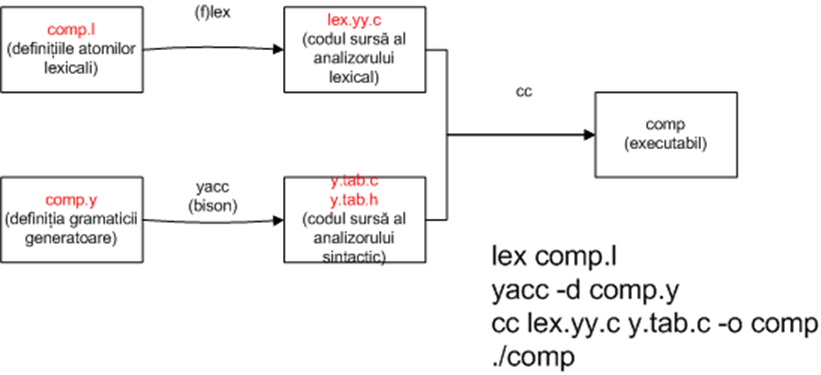
\includegraphics[width=\linewidth]{imgYacc1.png}
  	\label{fig:schema1}
\end{figure}

\end{itemize}
\end{frame}



\begin{frame}{Fişierul yacc/bison}
\begin{itemize}
	\item
	Fişierul yacc/bison are aceeşi structură ca şi fişierul lex/flex:
		\linebreak

	\begin{itemize}
	    	\item
		... Definiţii
			\linebreak
	
		\%\%
		\item
		... Reguli
			\linebreak
		\%\%
			\linebreak
	
		\item
		... Funcţii
	\end{itemize}
\end{itemize}
\end{frame}



\begin{frame}{Secţiunea definiţii}
\begin{itemize}
	\item
	Poate cuprinde:
	
	\item
	1. Cod C/C++

	\begin{itemize}
		\item<cir@1->
		Orice cod C/C++ scris între \%\{ şi \%\} este copiat ca atare în fişierul yacc/bison de ieşire.

		\item<cir@1->
		În această subsecţiune se definesc, de obicei, variabilele şi funcţiile care vor fi utilizate ulterior.
	\end{itemize}

	\item
	2. Definiţiile numelor atomilor lexicali

	\begin{itemize}
		\item<cir@1->
		În această subsecţiune se definesc numele atomilor lexicali pe care instrumentul de analiză sintactică care va fi generat îi recunoaşte.

		e.g. \%token NUME\_TOKEN

		\item<cir@1->
		La rularea yacc/bison, acesta generează un fişier header numit y.tab.h în care vor fi definite numele token-ilor folosind directiva define.

		e.g. \#define NUME\_TOKEN 258
	\end{itemize}

\end{itemize}
\end{frame}



\begin{frame}{Secţiunea definiţii}
\begin{itemize}
	\item[]
	\begin{itemize}
		\item<cir@1->
		În subsecţiunea de cod C/C++ a fişierului lex/flex corespunzător se va face include pentru fişierul y.tab.h, astfel încât analizorul lexical să poată utiliza denumirea atomilor lexicali aşteptată de către yacc/bison.

		\item<cir@1->
		Instrumentul de analiză sintactică generat apelează automat funcţia \textit{yylex()}. 
		
		\item<cir@1->
		La fiecare apel, aceasta trebuie să returneze numele unui atom lexical, aşa cum a fost acesta definit în fişierul yacc/bison.
	\end{itemize}

	\item
	3. Reguli de asociativitate

	\begin{itemize}
		\item<cir@1->
		Se definesc reguli privind asociativitatea şi prioritatea operatorilor.
	\end{itemize}

\end{itemize}
\end{frame}



\begin{frame}{Secţiunea reguli}
\begin{itemize}
	\item
	Cuprinde regulile de producţie ale gramaticii care defineşte limbajul ţintă.

	\item
	Fiecărei părţi drepte ale unei reguli de producţie poate să îi fie asociată o acţiune.

	\item
	Acţiunile sunt scrise în cod C/C++, şi apar între parantezele acolade.

	\item
	yacc/bison presupune că simbolul de start al gramaticii este primul simbol din secţiunea de reguli.

	\item
	Simbolul de start poate fi specificat şi explicit prin declaraţia {\color{red}\%start NETERMINAL}, în prima secţiune.

\end{itemize}
\end{frame}



\begin{frame}{Secţiunea funcţii}
\begin{itemize}
	\item
	Cuprinde definiţiile funcţiilor care vor fi utilizate.

	\item
	Funcţia main implicită pentru un compilator generat cu yacc/bison şi lex/flex este:
	\newline

	int main()
		\linebreak
		\{

		\begin{itemize}
			\item[]
			 yyparse();

			\item[]
			return 0;
		\end{itemize}

		\}
\end{itemize}
\end{frame}



\begin{frame}{Secţiunea funcţii}
\begin{itemize}
	\item
	Funcţia \textit{yyparse()} reprezintă analizorul sintactic generat. Ea apelează automat funcţia \textit{yylex()} ori de câte ori are nevoie de următorul atom lexical. 
\newline

	\item
	Fişierul lex/flex corespunzător nu va mai conţine funcţia main, deoarece cele două fişiere sursă generate pe rând de către yacc/bison şi respectiv de către lex/flex vor fi compilate împreună, şi deci este nevoie de o singură funcţie main.
\newline

	\item
	Variabilele şi funcţiile predefinite pentru lucrul cu fişiere (\textit{yyin, yyout, yywrap()}) sunt valabile şi pentru yacc/bison, putând fi utilizate exact în acelaşi mod ca şi pentru lex/flex.
\newline
\end{itemize}
\end{frame}



\begin{frame}{Ex1 din arhiva - Analiza sintactica}
\begin{itemize}
	\item
	Generarea unui analizor sintactic pentru limbajul expresiilor aritmetice.

	\item
	1. Definirea gramaticii pentru limbajul în cauză.

	\item[]
	Ex: S  $\rightarrow$  E ;

		\begin{itemize}
			\item[]
			       E  $\rightarrow$  E+E | E-E | E*E | E/E | (E) | NR
		\end{itemize}

	\item
	2. Scrierea fişierului pentru yacc/bison:

		\begin{itemize}
			\item<cir@1->
			      Definirea numelor atomilor lexicali (terminalelor din gramatică)
			\item<cir@1->
				Completarea regulilor de producţie
		\end{itemize}

\end{itemize}
\end{frame}



\begin{frame}{Ex1 din arhiva - Analiza sintactica}
\begin{itemize}
	\item[]
	\%\{

		\begin{itemize}
			\item[]
			      \#include <stdio.h>
			\item[]
				int EsteCorecta = 0;
		\end{itemize}

	\item[]
	\%\}
		\linebreak

	\item[]
	\%token TOK\_PLUS TOK\_MINUS TOK\_MULTIPLY TOK\_DIVIDE TOK\_LEFT TOK\_RIGHT TOK\_ERROR

	\item[]
	\%token TOK\_NUMBER
		\linebreak

	\item[]
	\%start S
		\linebreak

	\item[]
	\%left TOK\_PLUS TOK\_MINUS

	\item[]
	\%left TOK\_MULTIPLY TOK\_DIVIDE

\end{itemize}
\end{frame}



\begin{frame}{Ex1 din arhiva}
\begin{itemize}
	\item[]
	\%\%
	
	\item[]
	S : E ';' \{ EsteCorecta = 1; \}

		\begin{itemize}
			\item[]
			      ;
		\end{itemize}

	\item[]
	E : E TOK\_PLUS E

		\begin{itemize}
			\item[]
			      |

			\item[]
			E TOK\_MINUS E

			\item[]
			      |

			\item[]
			E TOK\_MULTIPLY E

			\item[]
			      |

			\item[]
			E TOK\_DIVIDE E

			\item[]
			      |

			\item[]
			TOK\_LEFT E TOK\_RIGHT

			\item[]
			      |

			\item[]
			TOK\_NUMBER

			\item[]
			      ;
		\end{itemize}

	\item[]
	\%\%

\end{itemize}
\end{frame}



\begin{frame}{Ex1 din arhiva}
\begin{itemize}
	\item[]
	int main()

	\item[]
	\{

		\begin{itemize}
			\item[]
			yyparse();

			\item[]
			if(EsteCorecta == 1)

			\item[]
			\{
				
				\begin{itemize}
					\item[]
					printf("CORECTA");
				\end{itemize}

			\item[]
			\}

			\item[]
			else

			\item[]
			\{
				
				\begin{itemize}
					\item[]
					printf("INCORECTA");
				\end{itemize}

			\item[]
			\}

			\item[]
			return 0;
		\end{itemize}

	\item[]
	\}
		\linebreak

	\item[]
	int yyerror(const char *msg)

	\item[]
	\{

		\begin{itemize}
			\item[]
			printf("Error: \%s", msg);

			\item[]
			return 1;
		\end{itemize}

	\item[]
	\}

\end{itemize}
\end{frame}



\begin{frame}{Ex1 din arhiva - Analiza sintactica}
\begin{itemize}
	\item
	3. Scrierea fişierului pentru lex/flex, având în vedere atomii lexicali (terminalele gramaticii) definiti in fisierul yacc/bison

\end{itemize}
\end{frame}



\begin{frame}{Ex1 din arhiva}
\begin{itemize}
	\item[]
	\%\{
		
		\begin{itemize}
			\item[]
					\#include "y.tab.h"
		\end{itemize}

	\item[]
	\%\}

	\item[]
	\%\%

	\item[]
	"+" \hspace{1.55cm} \{ return TOK\_PLUS; \}

	\item[]
	"-" \hspace{1.7cm} \{ return TOK\_MINUS; \}

	\item[]
	"*" \hspace{1.65cm} \{ return TOK\_MULTIPLY; \}

	\item[]
	"/" \hspace{1.65cm} \{ return TOK\_DIVIDE; \}

	\item[]
	"(" \hspace{1.65cm} \{ return TOK\_LEFT; \}

	\item[]
	")" \hspace{1.65cm} \{ return TOK\_RIGHT; \}

	\item[]
	";" \hspace{1.7cm} \{ return ';'; \}

	\item[]
	{[1-9][0-9]}*|0 \hspace{0.25cm} \{ return TOK\_NUMBER; \}

	\item[]
	. \hspace{2cm} \{ return TOK\_ERROR; \}

	\item[]
	\%\%

\end{itemize}
\end{frame}



\begin{frame}{Ex1 din arhiva - Analiza sintactica}
\begin{itemize}
	\item
	4. Generarea executabilului.

	\item[]
	yacc –d ex.y

	\item[]
	lex ex.l

	\item[]
	cc lex.yy.c y.tab.c –o ex –lfl
		\linebreak

	\item
	5. Execuţia

	\item[]
	./ex <in.txt >out.txt

\end{itemize}
\end{frame}



\begin{frame}{Funcţionarea yacc/bison}
\begin{itemize}
	\item
	Punctul de intrare în analiză pentru analizoarele sintactice generate cu ajutorul lui yacc este funcţia yyparse(). 

	\item
	Ori de câte ori analizorul sintactic are nevoie de următorul atom lexical din intrare, el apelează funcţia yylex(). Aceasta îi întoarce identificatorul următorului atom lexical sau o valoare care arată că nu mai sunt atomi lexicali în intrare.


	\item
	Identificatorii atomilor lexicali sunt cei definiţi prin \%token.

	\item
	Analizoarele sintactice generate de către yacc implementează o analiză sintactică ascendentă: prin operaţii shift-reduce încearcă să reducă succesiunea de atomi lexicali la simbolul de start al gramaticii.

\end{itemize}
\end{frame}



\begin{frame}{Funcţionarea yacc/bison}
\begin{itemize}
	\item
	Pe măsură ce yacc citeşte atomi lexicali, îi salvează într-o stivă (shift). 

	\item
	În momentul în care ultimii n atomi lexicali de pe vârful stivei se potrivesc cu partea dreptă a unei reguli de producţie din secţiunea de reguli a fişierului *.y, aceştia pot fi grupaţi împreună şi înlocuiţi cu partea stângă a regulii de producţie respective (reduce).

	\item
	Yacc nu face însă o reducere imediat ce ultimii n atomi lexicali se potrivesc părţii drepte ale unei reguli de producţie.

\end{itemize}
\end{frame}



\begin{frame}{Funcţionarea yacc (bison)}
\begin{itemize}
	\item
	Atunci când un atom lexical este întors de către yylex(), el nu este imediat shiftat pe stivă, ci devine mai întâi  {\color{red}lookahead token} (atomul lexical următor, aşa cum este el folosit şi în analiza LL(1)).
 
	\item
	Atunci când este posibilă o reducere, yacc se uită la valoarea lui lookahead token (care nu se află în stivă, ci reprezintă următorul atom lexical care va fi shiftat).

	\item
	În funcţie de valoarea sa, yacc face una sau mai multe reduceri.

	\item
	Dacă nu mai este posibilă nicio reducere, lookahead token este shiftat pe stivă, se cere lui yykex() următorul atom lexical, iar atomul lexical întors de yylex() devine lookahead token.

	\item
	Lookahead token este stocat în variabila {\color{red} yychar} (variabilă predefinită). Când această variabilă nu conţine un atom lexical, ea are valoarea {\color{red}YYEMPTY}.

\end{itemize}
\end{frame}



\begin{frame}{Funcţionarea yacc/bison}
\begin{columns}
\begin{column}{0.5\textwidth}
\begin{itemize}
	\item
	E $\rightarrow$ E + E

	\item
	E $\rightarrow$ E - E

	\item
	E $\rightarrow$ E * E

	\item
	E $\rightarrow$ E / E

	\item
	E $\rightarrow$ E \textsuperscript{$\wedge$} E

	\item
	E $\rightarrow$ (E)

	\item
	E $\rightarrow$ NR !

	\item
	E $\rightarrow$ NR

\end{itemize}
\end{column}

\begin{column}{0.3\textwidth}
\begin{tabular}{cc|c|} \cline{1-2}
\multicolumn{1}{|c}{\textbf{Intrare}} & {\hspace{0.4cm} 1+2!} \\ \cline{1-2}
\multicolumn{1}{|c|}{\textbf{Stiva} \hspace{0.5cm}} &   \cline{1-2}
\multicolumn{1}{|c|} \textepsilon \\ \cline{1-1}

\end{tabular}
\end{column}

\end{columns}
\end{frame}



\begin{frame}{Funcţionarea yacc/bison}
\begin{columns}
\begin{column}{0.5\textwidth}
\begin{itemize}
	\item
	E $\rightarrow$ E + E

	\item
	E $\rightarrow$ E - E

	\item
	E $\rightarrow$ E * E

	\item
	E $\rightarrow$ E / E

	\item
	E $\rightarrow$ E \textsuperscript{$\wedge$} E

	\item
	E $\rightarrow$ (E)

	\item
	E $\rightarrow$ NR !

	\item
	E $\rightarrow$ NR

\end{itemize}
\end{column}

\begin{column}{0.3\textwidth}
\begin{tabular}{cc|c|} \cline{1-2}
\multicolumn{1}{|c}{\textbf{Intrare}} & {\hspace{0.4cm} +2!} \\ \cline{1-2}
\multicolumn{1}{|c|}{\textbf{Stiva} \hspace{0.5cm}} &   \cline{1-2}
\multicolumn{1}{|c|} {NR} \\ \cline{1-1}
\end{tabular}

\end{column}
\end{columns}
\end{frame}



\begin{frame}{Funcţionarea yacc/bison}
\begin{columns}
\begin{column}{0.5\textwidth}
\begin{itemize}
	\item
	E $\rightarrow$ E + E

	\item
	E $\rightarrow$ E - E

	\item
	E $\rightarrow$ E * E

	\item
	E $\rightarrow$ E / E

	\item
	E $\rightarrow$ E \textsuperscript{$\wedge$} E

	\item
	E $\rightarrow$ (E)

	\item
	E $\rightarrow$ NR !

	\item
	E $\rightarrow$ NR

\end{itemize}
\end{column}

\begin{column}{0.3\textwidth}
\begin{tabular}{cc|c|} \cline{1-2}
\multicolumn{1}{|c}{\textbf{Intrare}} & {\hspace{0.4cm} +2!} \\ \cline{1-2}
\multicolumn{1}{|c|}{\textbf{Stiva} \hspace{0.5cm}} &   \cline{1-2}
\multicolumn{1}{|c|} {E} \\ \cline{1-1}
\end{tabular}

\end{column}
\end{columns}
\end{frame}



\begin{frame}{Funcţionarea yacc/bison}
\begin{columns}
\begin{column}{0.5\textwidth}
\begin{itemize}
	\item
	E $\rightarrow$ E + E

	\item
	E $\rightarrow$ E - E

	\item
	E $\rightarrow$ E * E

	\item
	E $\rightarrow$ E / E

	\item
	E $\rightarrow$ E \textsuperscript{$\wedge$} E

	\item
	E $\rightarrow$ (E)

	\item
	E $\rightarrow$ NR !

	\item
	E $\rightarrow$ NR

\end{itemize}
\end{column}

\begin{column}{0.3\textwidth}
\begin{tabular}{cc|c|} \cline{1-2}
\multicolumn{1}{|c}{\textbf{Intrare}} & {\hspace{0.4cm} +2!} \\ \cline{1-2}
\multicolumn{1}{|c|}{\textbf{Stiva} \hspace{0.5cm}} &   \cline{1-2}
\multicolumn{1}{|c|} {+} \\
\multicolumn{1}{|c|} {E} \\ \cline{1-1}
\end{tabular}

\end{column}
\end{columns}
\end{frame}



\begin{frame}{Funcţionarea yacc/bison}
\begin{columns}
\begin{column}{0.5\textwidth}
\begin{itemize}
	\item
	E $\rightarrow$ E + E

	\item
	E $\rightarrow$ E - E

	\item
	E $\rightarrow$ E * E

	\item
	E $\rightarrow$ E / E

	\item
	E $\rightarrow$ E \textsuperscript{$\wedge$} E

	\item
	E $\rightarrow$ (E)

	\item
	E $\rightarrow$ NR !

	\item
	E $\rightarrow$ NR

\end{itemize}
\end{column}

\begin{column}{0.3\textwidth}
\begin{tabular}{cc|c|} \cline{1-2}
\multicolumn{1}{|c}{\textbf{Intrare}} & {\hspace{0.4cm} !} \\ \cline{1-2}
\multicolumn{1}{|c|}{\textbf{Stiva} \hspace{0.5cm}} &   \cline{1-2}
\multicolumn{1}{|c|} {NR} \\
\multicolumn{1}{|c|} {+} \\
\multicolumn{1}{|c|} {E} \\ \cline{1-1}
\end{tabular}

\end{column}
\end{columns}
\end{frame}



\begin{frame}{Funcţionarea yacc/bison}
\begin{columns}
\begin{column}{0.5\textwidth}
\begin{itemize}
	\item
	E $\rightarrow$ E + E

	\item
	E $\rightarrow$ E - E

	\item
	E $\rightarrow$ E * E

	\item
	E $\rightarrow$ E / E

	\item
	E $\rightarrow$ E \textsuperscript{$\wedge$} E

	\item
	E $\rightarrow$ (E)

	\item
	E $\rightarrow$ NR !

	\item
	E $\rightarrow$ NR

\end{itemize}
\end{column}

\begin{column}{0.3\textwidth}
\begin{tabular}{cc|c|} \cline{1-2}
\multicolumn{1}{|c}{\textbf{Intrare}} & {\hspace{0.4cm} !} \\ \cline{1-2}
\multicolumn{1}{|c|}{\textbf{Stiva} \hspace{0.5cm}} &   \cline{1-2}
\multicolumn{1}{|c|} {E} \\
\multicolumn{1}{|c|} {+} \\
\multicolumn{1}{|c|} {E} \\ \cline{1-1}
\end{tabular}

\end{column}
\end{columns}
\end{frame}



\begin{frame}{Funcţionarea yacc/bison}
\begin{columns}
\begin{column}{0.5\textwidth}
\begin{itemize}
	\item
	E $\rightarrow$ E + E

	\item
	E $\rightarrow$ E - E

	\item
	E $\rightarrow$ E * E

	\item
	E $\rightarrow$ E / E

	\item
	E $\rightarrow$ E \textsuperscript{$\wedge$} E

	\item
	E $\rightarrow$ (E)

	\item
	E $\rightarrow$ NR !

	\item
	E $\rightarrow$ NR

\end{itemize}
\end{column}

\begin{column}{0.3\textwidth}
\begin{tabular}{cc|c|} \cline{1-2}
\multicolumn{1}{|c}{\textbf{Intrare}} & {\hspace{0.4cm} !} \\ \cline{1-2}
\multicolumn{1}{|c|}{\textbf{Stiva} \hspace{0.5cm}} &   \cline{1-2}
\multicolumn{1}{|c|} {E} \\ \cline{1-1}
\end{tabular}

\end{column}
\end{columns}
\end{frame}



\begin{frame}{Funcţionarea yacc/bison}
\begin{columns}
\begin{column}{0.5\textwidth}
\begin{itemize}
	\item
	E $\rightarrow$ E + E

	\item
	E $\rightarrow$ E - E

	\item
	E $\rightarrow$ E * E

	\item
	E $\rightarrow$ E / E

	\item
	E $\rightarrow$ E \textsuperscript{$\wedge$} E

	\item
	E $\rightarrow$ (E)

	\item
	E $\rightarrow$ NR !

	\item
	E $\rightarrow$ NR

\end{itemize}
\end{column}

\begin{column}{0.3\textwidth}
\begin{tabular}{cc|c|} \cline{1-2}
\multicolumn{1}{|c}{\textbf{Intrare}} & {\hspace{0.4cm} \textepsilon} \\ \cline{1-2}
\multicolumn{1}{|c|}{\textbf{Stiva} \hspace{0.5cm}} &   \cline{1-2}
\multicolumn{1}{|c|} {!} \\
\multicolumn{1}{|c|} {E} \\ \cline{1-1}
\\
\end{tabular}
	
Propoziţia este incorectă?


\end{column}
\end{columns}
\end{frame}



\begin{frame}{Funcţionarea yacc/bison}
\begin{columns}
\begin{column}{0.5\textwidth}
\begin{itemize}
	\item
	E $\rightarrow$ E + E

	\item
	E $\rightarrow$ E - E

	\item
	E $\rightarrow$ E * E

	\item
	E $\rightarrow$ E / E

	\item
	E $\rightarrow$ E \textsuperscript{$\wedge$} E

	\item
	E $\rightarrow$ (E)

	\item
	E $\rightarrow$ NR !

	\item
	E $\rightarrow$ NR

\end{itemize}
\end{column}

\begin{column}{0.3\textwidth}
\begin{tabular}{cc|c|} \cline{1-2}
\multicolumn{1}{|c}{\textbf{Intrare}} & {\hspace{0.4cm} 1+2!} \\ \cline{1-2}
\multicolumn{1}{|c}{\textbf{Lookahead}} & {\hspace{0.4cm} \textepsilon} \\  \cline{1-2}
\\ \cline{1-1}
\multicolumn{1}{|c|}{\textbf{Stiva} \hspace{0.5cm}} &  \cline{1-2}
\multicolumn{1}{|c|} {\textepsilon} \\ \cline{1-1}
\end{tabular}

\end{column}
\end{columns}
\end{frame}



\begin{frame}{Funcţionarea yacc/bison}
\begin{columns}
\begin{column}{0.5\textwidth}
\begin{itemize}
	\item
	E $\rightarrow$ E + E

	\item
	E $\rightarrow$ E - E

	\item
	E $\rightarrow$ E * E

	\item
	E $\rightarrow$ E / E

	\item
	E $\rightarrow$ E \textsuperscript{$\wedge$} E

	\item
	E $\rightarrow$ (E)

	\item
	E $\rightarrow$ NR !

	\item
	E $\rightarrow$ NR

\end{itemize}
\end{column}

\begin{column}{0.3\textwidth}
\begin{tabular}{cc|c|} \cline{1-2}
\multicolumn{1}{|c}{\textbf{Intrare}} & {\hspace{0.4cm} +2!} \\ \cline{1-2}
\multicolumn{1}{|c}{\textbf{Lookahead}} & {\hspace{0.4cm} NR} \\  \cline{1-2}
\\ \cline{1-1}
\multicolumn{1}{|c|}{\textbf{Stiva} \hspace{0.5cm}} &  \cline{1-2}
\multicolumn{1}{|c|} {\textepsilon} \\ \cline{1-1}
\end{tabular}

\end{column}
\end{columns}
\end{frame}



\begin{frame}{Funcţionarea yacc/bison}
\begin{columns}
\begin{column}{0.5\textwidth}
\begin{itemize}
	\item
	E $\rightarrow$ E + E

	\item
	E $\rightarrow$ E - E

	\item
	E $\rightarrow$ E * E

	\item
	E $\rightarrow$ E / E

	\item
	E $\rightarrow$ E \textsuperscript{$\wedge$} E

	\item
	E $\rightarrow$ (E)

	\item
	E $\rightarrow$ NR !

	\item
	E $\rightarrow$ NR

\end{itemize}
\end{column}

\begin{column}{0.3\textwidth}
\begin{tabular}{cc|c|} \cline{1-2}
\multicolumn{1}{|c}{\textbf{Intrare}} & {\hspace{0.4cm} 2!} \\ \cline{1-2}
\multicolumn{1}{|c}{\textbf{Lookahead}} & {\hspace{0.4cm} +} \\  \cline{1-2}
\\ \cline{1-1}
\multicolumn{1}{|c|}{\textbf{Stiva} \hspace{0.5cm}} &  \cline{1-2}
\multicolumn{1}{|c|} {NR} \\ \cline{1-1}
\end{tabular}

\end{column}
\end{columns}
\end{frame}



\begin{frame}{Funcţionarea yacc/bison}
\begin{columns}
\begin{column}{0.5\textwidth}
\begin{itemize}
	\item
	E $\rightarrow$ E + E

	\item
	E $\rightarrow$ E - E

	\item
	E $\rightarrow$ E * E

	\item
	E $\rightarrow$ E / E

	\item
	E $\rightarrow$ E \textsuperscript{$\wedge$} E

	\item
	E $\rightarrow$ (E)

	\item
	E $\rightarrow$ NR !

	\item
	E $\rightarrow$ NR

\end{itemize}
\end{column}

\begin{column}{0.3\textwidth}
\begin{tabular}{cc|c|} \cline{1-2}
\multicolumn{1}{|c}{\textbf{Intrare}} & {\hspace{0.4cm} 2!} \\ \cline{1-2}
\multicolumn{1}{|c}{\textbf{Lookahead}} & {\hspace{0.4cm} +} \\  \cline{1-2}
\\ \cline{1-1}
\multicolumn{1}{|c|}{\textbf{Stiva} \hspace{0.5cm}} &  \cline{1-2}
\multicolumn{1}{|c|} {E} \\ \cline{1-1}
\end{tabular}

\end{column}
\end{columns}
\end{frame}



\begin{frame}{Funcţionarea yacc/bison}
\begin{columns}
\begin{column}{0.5\textwidth}
\begin{itemize}
	\item
	E $\rightarrow$ E + E

	\item
	E $\rightarrow$ E - E

	\item
	E $\rightarrow$ E * E

	\item
	E $\rightarrow$ E / E

	\item
	E $\rightarrow$ E \textsuperscript{$\wedge$} E

	\item
	E $\rightarrow$ (E)

	\item
	E $\rightarrow$ NR !

	\item
	E $\rightarrow$ NR

\end{itemize}
\end{column}

\begin{column}{0.3\textwidth}
\begin{tabular}{cc|c|} \cline{1-2}
\multicolumn{1}{|c}{\textbf{Intrare}} & {\hspace{0.4cm} !} \\ \cline{1-2}
\multicolumn{1}{|c}{\textbf{Lookahead}} & {\hspace{0.4cm} NR} \\  \cline{1-2}
\\ \cline{1-1}
\multicolumn{1}{|c|}{\textbf{Stiva} \hspace{0.5cm}} &  \cline{1-2}
\multicolumn{1}{|c|} {+} \\
\multicolumn{1}{|c|} {E} \\ \cline{1-1}
\end{tabular}

\end{column}
\end{columns}
\end{frame}



\begin{frame}{Funcţionarea yacc/bison}
\begin{columns}
\begin{column}{0.5\textwidth}
\begin{itemize}
	\item
	E $\rightarrow$ E + E

	\item
	E $\rightarrow$ E - E

	\item
	E $\rightarrow$ E * E

	\item
	E $\rightarrow$ E / E

	\item
	E $\rightarrow$ E \textsuperscript{$\wedge$} E

	\item
	E $\rightarrow$ (E)

	\item
	E $\rightarrow$ NR !

	\item
	E $\rightarrow$ NR

\end{itemize}
\end{column}

\begin{column}{0.3\textwidth}
\begin{tabular}{cc|c|} \cline{1-2}
\multicolumn{1}{|c}{\textbf{Intrare}} & {\hspace{0.4cm} \textepsilon} \\ \cline{1-2}
\multicolumn{1}{|c}{\textbf{Lookahead}} & {\hspace{0.4cm} !} \\  \cline{1-2}
\\ \cline{1-1}
\multicolumn{1}{|c|}{\textbf{Stiva} \hspace{0.5cm}} &  \cline{1-2}
\multicolumn{1}{|c|} {NR} \\
\multicolumn{1}{|c|} {+} \\
\multicolumn{1}{|c|} {E} \\ \cline{1-1}
\end{tabular}

\end{column}
\end{columns}
\end{frame}



\begin{frame}{Funcţionarea yacc/bison}
\begin{columns}
\begin{column}{0.5\textwidth}
\begin{itemize}
	\item
	E $\rightarrow$ E + E

	\item
	E $\rightarrow$ E - E

	\item
	E $\rightarrow$ E * E

	\item
	E $\rightarrow$ E / E

	\item
	E $\rightarrow$ E \textsuperscript{$\wedge$} E

	\item
	E $\rightarrow$ (E)

	\item
	E $\rightarrow$ NR !

	\item
	E $\rightarrow$ NR

\end{itemize}
\end{column}

\begin{column}{0.3\textwidth}
\begin{tabular}{cc|c|} \cline{1-2}
\multicolumn{1}{|c}{\textbf{Intrare}} & {\hspace{0.4cm} \textepsilon} \\ \cline{1-2}
\multicolumn{1}{|c}{\textbf{Lookahead}} & {\hspace{0.4cm} \textepsilon} \\  \cline{1-2}
\\ \cline{1-1}
\multicolumn{1}{|c|}{\textbf{Stiva} \hspace{0.5cm}} &  \cline{1-2}
\multicolumn{1}{|c|} {!} \\
\multicolumn{1}{|c|} {NR} \\
\multicolumn{1}{|c|} {+} \\
\multicolumn{1}{|c|} {E} \\ \cline{1-1}
\end{tabular}

\end{column}
\end{columns}
\end{frame}



\begin{frame}{Funcţionarea yacc/bison}
\begin{columns}
\begin{column}{0.5\textwidth}
\begin{itemize}
	\item
	E $\rightarrow$ E + E

	\item
	E $\rightarrow$ E - E

	\item
	E $\rightarrow$ E * E

	\item
	E $\rightarrow$ E / E

	\item
	E $\rightarrow$ E \textsuperscript{$\wedge$} E

	\item
	E $\rightarrow$ (E)

	\item
	E $\rightarrow$ NR !

	\item
	E $\rightarrow$ NR

\end{itemize}
\end{column}

\begin{column}{0.3\textwidth}
\begin{tabular}{cc|c|} \cline{1-2}
\multicolumn{1}{|c}{\textbf{Intrare}} & {\hspace{0.4cm} \textepsilon} \\ \cline{1-2}
\multicolumn{1}{|c}{\textbf{Lookahead}} & {\hspace{0.4cm} \textepsilon} \\  \cline{1-2}
\\ \cline{1-1}
\multicolumn{1}{|c|}{\textbf{Stiva} \hspace{0.5cm}} &  \cline{1-2}
\multicolumn{1}{|c|} {E} \\
\multicolumn{1}{|c|} {+} \\
\multicolumn{1}{|c|} {E} \\ \cline{1-1}
\end{tabular}

\end{column}
\end{columns}
\end{frame}



\begin{frame}{Funcţionarea yacc/bison}
\begin{columns}
\begin{column}{0.5\textwidth}
\begin{itemize}
	\item
	E $\rightarrow$ E + E

	\item
	E $\rightarrow$ E - E

	\item
	E $\rightarrow$ E * E

	\item
	E $\rightarrow$ E / E

	\item
	E $\rightarrow$ E \textsuperscript{$\wedge$} E

	\item
	E $\rightarrow$ (E)

	\item
	E $\rightarrow$ NR !

	\item
	E $\rightarrow$ NR

\end{itemize}
\end{column}

\begin{column}{0.3\textwidth}
\begin{tabular}{cc|c|} \cline{1-2}
\multicolumn{1}{|c}{\textbf{Intrare}} & {\hspace{0.4cm} \textepsilon} \\ \cline{1-2}
\multicolumn{1}{|c}{\textbf{Lookahead}} & {\hspace{0.4cm} \textepsilon} \\  \cline{1-2}
\\ \cline{1-1}
\multicolumn{1}{|c|}{\textbf{Stiva} \hspace{0.5cm}} &  \cline{1-2}
\multicolumn{1}{|c|} {E} \\ \cline{1-1}
\\
\end{tabular}

Propoziţia este corectă.

\end{column}
\end{columns}
\end{frame}



\begin{frame}{Precedenţa şi asociativitatea operatorilor}
\begin{itemize}
	\item
	Asociativitatea determină modul în care se grupează utilizările repetate ale aceluiaşi operator.

	\item
	Precedenţa arată modul în care un operator se grupează cu alţi operatori.

	\item
	Asociativitatea atomilor lexicali ai gramaticii se definesc cu ajutorul lui:

	\begin{itemize}
		\item<cir@1->
		{\color{red}\%left NUME\_TOKEN} – asociativitate stânga (pt x op y op z se grupează mai întâi x cu y).

		\item<cir@1->
		{\color{red}\%right NUME\_TOKEN} – asociativitate dreapta (pt x op y op z se grupează mai întâi y cu z).
	
		\item<cir@1->
		{\color{red}\%nonassoc NUME\_TOKEN} – nicio asociativitate: operatorul nu se poate afla de mai multe ori în acelaşi rând (x op y op z va fi considerată incorectă sintactic).

	\end{itemize}	

\end{itemize}
\end{frame}



\begin{frame}{Precedenţa şi asociativitatea operatorilor}
\begin{itemize}
	\item
	Precedenţa atomilor lexicali ai gramaticii rezultă din modul în care a fost definită asociativitatea lor:

	\begin{itemize}
		\item[]
		- Atomii lexicali a căror asociativitate a fost definită în aceeaşi declaraţie \%left, \%right sau \%nonassoc au aceeaşi precedenţă şi se grupează potrivit asociativităţii lor.
	
		\item[]
		- Atomii lexicali a căror asociativitate a fost definită în declaraţii diferite au precedenţe diferite, după cum urmează: cel pentru care a fost definită ultima data asociativitatea are precedenţa cea mai mare, iar cel pentru care asociativitatea a fost definită prima dată are precedenţa cea mai mică.
	\end{itemize}

	\item
	Ultimul pentru care a fost declarată asociativitatea va fi grupat primul, iar primul pentru care a fost declarată asociativitatea va fi grupat ultimul.

\end{itemize}
\end{frame}



\begin{frame}{Precedenţa şi asociativitatea operatorilor}
\begin{itemize}
	\item
	Ex:

	\begin{itemize}
		\item[]
		\% left ‘+’ ‘-’

		\item[]
		\% left ‘*’ ‘/’

		\item[]
		\%left ‘!’

	\end{itemize}	

	\item
	Rezultă:

	\begin{itemize}
		\item[]
		1. Toate terminalele au asociativitate stânga.

		\item[]
		2. ! Are precedenţa mai mare decât * şi /, iar * şi / au precedenţa mai mare decât + şi -.

	\end{itemize}	

\end{itemize}
\end{frame}



\begin{frame}{Precedenţa contextuală}
\begin{itemize}
	\item
	Precedenţa unui operator, care depinde de context, se specifică cu ajutorul declaraţiei {\color{red}\%prec}. 

	\item
	Ex: Operatorul minus (-) poate fi operator binar (reprezintă scăderea) sau operator unar (reprezintă semnul unui număr). Atunci când este semn, minus are precedenţa mai mare decât atunci când reprezintă scăderea.

	\begin{itemize}
		\item[]
		\%left ‘-’

		\item[]
		\%left UMINUS

		\item[]
		E  $\rightarrow$  E ‘-’ E

		\item[]
		\hspace{0.7cm} | ‘-’ E {\color{red}\%prec UMINUS}   

		\item[]
		\hspace{0.7cm} | NR

	\end{itemize}

	\item
	Regula ‘-’ E are aceeaşi precedenţă ca şi UMINUS, deci mai mare decât ‘-’, conform declaraţiilor de asociativitate.

\end{itemize}
\end{frame}



\begin{frame}{Conflicte shift/reduce}
\begin{itemize}
	\item
	Ex:

	\begin{itemize}
		\item[]
		DECL\_IF  $\rightarrow$  if EXP then DECL

		\item[]
		\hspace{1.95cm} |

		\item[]
		\hspace{1.95cm} if EXP then DECL else DECL

	\end{itemize}	

	\item
	Pe parcursul analizei sintactice, după ce atomii lexicali “if EXP then DECL” sunt shiftaţi pe stivă, “else” devine lookahead token.

	\item
	În momentul acela există două posibilităţi de continuare: 

	\begin{itemize}
		\item[]
		1. Să reducă “if EXP then DECL” la DECL\_IF.

		\item[]
		2. Să îl shifteze pe “else” pe stivă, pentru ca ulterior să reducă “if EXP then DECL else DECL” la DECL\_IF.

	\end{itemize}

\end{itemize}
\end{frame}



\begin{frame}{Conflicte shift/reduce}
\begin{itemize}
	\item
	Conform regulilor de producţie, ambele operaţii posibile (atât operaţia shift, cât şi operaţia reduce) sunt corecte. Rezultă {\color{red}un conflict shift/reduce}.

	\item
	Modul implicit în care yacc rezolvă aceste conflicte este executând operaţia shift.

	\item
	Totuşi, utilizatorul va fi imformat asupra conflictului printr-un mesaj de atenţionare.

	\item
	Pentru a evita aceste mesaje de atenţionare relativ la conflictele shift/reduce, se poate utiliza declaraţia {\color{red}\%expect n}: yacc nu va genera mesaje de atenţionare atâta timp cât numărul de conflicte shift/reduce este exact n.

\end{itemize}
\end{frame}



\begin{frame}{Conflicte shift/reduce}
\begin{itemize}
	\item
	Un alt mod derezolvare a acestor conflicte este utilizarea precedenţei contextuale (precedenţa unui operator depinde de contextul în care acesta se află).

	\item
	Ex:

	
	\begin{itemize}
		\item<cir@1->
		1. Definim un atom lexical ifx, care să reprezinte instrucţiunea if fără else.

		\item<cir@1->
		2. Declarăm ifx şi else ca fiind neasociative, şi astfel încât else să aibă precedenţa mai mare decât ifx.

		\item[]
		\%nonassoc ifx

		\item[]
		\%nonassoc else

		\item[]
		(Deoarece asociativitatea lui else este definită după cea a lui ifx, atunci else are precedenţă mai mare decât ifx.)

	\end{itemize}

\end{itemize}
\end{frame}



\begin{frame}{Conflicte shift/reduce}
\begin{itemize}
	\item[]
	
	\begin{itemize}
		\item<cir@1->
		3. Utilizăm declaraţia de precedenţă contextuală {\color{red}\%prec} pentru a specifica că if fără else are aceeaşi precedenţă ca şi ifx:

		\begin{itemize}
			\item[]
			DECL\_IF  $\rightarrow$  if EXP then DECL {\color{red}\%prec ifx}

			\item[]
			\hspace{1.85cm} |

			\item[]
			\hspace{1.85cm} if EXP then DECL else DECL
				\linebreak

		\end{itemize}

		\item[]
		În consecinţă, “if EXP then DECL” are aceeaşi precedenţă ca şi ifx, adică mai mică decât a lui else. Prin urmare, yacc va face shift, deplasând pe else pe stivă.

	\end{itemize}

\end{itemize}
\end{frame}



\begin{frame}{Conflicte reduce/reduce}
\begin{itemize}
	\item
	Un conflict reducere/reducere apare atunci când pentru reducerea unei secvenţe de atomi lexicali pot fi aplicate mai multe reguli de producţie.

	\item
	Ex:

	\begin{itemize}
		\item[]
		propoziţie  $\rightarrow$  \textepsilon

		\item[]
		\hspace{1.45cm}  $\rightarrow$  cuvântul\_poate

		\item[]
		\hspace{1.45cm}  $\rightarrow$  propoziţie cuvânt
	
		\item[]
		cuvântul\_poate  $\rightarrow$  \textepsilon

		\item[]
		\hspace{2.35cm}  $\rightarrow$  cuvânt

	\end{itemize}

	\item
	Un cuvânt poate fi redus la o propoziţie prin mai multe căi:

	\begin{itemize}
		\item[]
		1. Un cuvânt este redus la cuvântul\_poate, iar acesta este redus la o propoziţie.

		\item[]
		2. \textepsilon,  este redus la propoziţie, iar propoziţie împreună cu cuvânt este redus la propoziţie
	\end{itemize}

\end{itemize}
\end{frame}



\begin{frame}{Conflicte reduce/reduce}
\begin{itemize}
	\item
	Acest tip de conflicte nu afectează validitatea analizei, indiferent de reducerile utilizate: o propoziţie validă va fi considerată validă, iar una incorectă va fi găsită ca fiind incorectă.

	\item
	Ceea ce diferă este însă ieşirea programului: aceasta depinde de acţiunea asociată fiecărei reguli de producţie. Deci, în funcţie de regula utilizată la reducere se va executa o altă acţiune.

	\item
	Yacc rezolvă implicit aceste conflicte aplicând cu prioritate regula care apare prima în secţiunea de reguli a fişierului *.y.

	\item
	Modul implicit de rezolvare a acestor conflicte este, de obicei, riscant.

	\item
	Cel mai corect este studierea regulilor de producţie ale gramaticii şi eliminarea manuală a conflictelor.

\end{itemize}
\end{frame}



\begin{frame}{Tratarea erorilor}
\begin{itemize}
	\item
	Comportamentul implicit al yacc în momentul în care întâlneşte o eroare sintactică este să oprească analiza, afişând un mesaj corespunzător.

	\item
	În majoritatea cazurilor ar fi mult mai folositor ca yacc să continue analiza sintactică pentru a descoperi toate erorile din intrare.

	\item
	Pentru a permite utilizatorului să controleze procesul de tratare a erorilor, yacc pune la dispoziţie un atom lexical special cu numele {\color{red}error}.

	\item
	Acesta poate fi utilizat în secţiunea de reguli a fişierului *.y, la scrierea regulilor de producţie ale gramaticii care defineşte limbajul ţintă, pentru a arăta locurile în care se aşteaptă să apară erori.

\end{itemize}
\end{frame}



\begin{frame}{Tratarea erorilor}
\begin{itemize}
	\item
	La întâlnirea unei erori sintactice, yacc scoate de pe stivă câte un element, până în momentul în care atomul lexical {\color{red}error} este legal (apare într-un context care corespunde regulilor de producţie ale gramaticii).

	\item
	Apoi, el se comportă ca şi cum error ar fi lookahead token-ul curent, şi execută acţiunea corespunzătoare.

	\item
	Lookahead token este apoi resetat la atomul lexical care a generat eroarea.

	\item
	După detectarea unei erori, analizorul sintactic rămâne în starea error până când trei atomi lexicali sunt citiţi şi deplasaţi cu succes pe stivă.

	\item
	Dacă pe timpul în care analizorul se află în starea error este detectată o nouă eroare, atunci nu se mai afişază un mesaj de eroare, iar atomul lexical de intrare este şters în mod silenţios.

\end{itemize}
\end{frame}



\begin{frame}{Tratarea erorilor}
\begin{itemize}
	\item
	O regulă de forma:

	\item[]
	\hspace{2.9cm}{\color{red}Instrucţiune : error ‘;’}

	\item
	Înseamnă că la apariţia unei erori analizorul sintactic va încerca să treacă peste instrucţiunea care a cauzat eroarea, şi va face acest lucru sărind până la următorul ‘;’.

	\item
	Toţi atomii lexicali de după error, şi înainte de ‘;’ vor fi eliminaţi, deoarece nu pot fi deplasaţi pe stivă.

	\item
	La întâlnirea lui ‘;’ {\color{red}error ‘;’} vor fi reduse la {\color{red}Instrucţiune} şi se va executa acţiunea de “curăţare” asociată.

\end{itemize}
\end{frame}



\begin{frame}{Tratarea erorilor}
\begin{itemize}
	\item
	Se pot utiliza şi reguli generale, de forma:

	\item[]
	\hspace{2.9cm}{\color{red}Instrucţiune : error}

	\item
	Dar în acest caz analizorul sintactic va încerca să treacă peste instrucţiunea care a cauzat eroarea într-un mod la fel de general: folosind analizorul lexical, el va căuta următorul grup de trei atomi lexicali care ar putea urma legal unei instrucţiuni, şi va relua analiza începând cu primul dintre aceştia.

	\item
	Dacă începutul unei instrucţiuni nu este suficient de diferit faţă de ceea ce ar putea apărea în interiorul acesteia, yacc ar putea să găseasc un start fals în interiorul instrucţiunii respective, şi să genereze o a doua eroare, deşi este vorba de aceeaşi.

\end{itemize}
\end{frame}



\begin{frame}[shrink=10]{Tratarea erorilor}
\begin{itemize}
	\item
	yyerrok;

	\begin{itemize}
		\item<cir@1->
		Macro care permite forţarea analizorului sintactic să creadă că s-a revenit complet dintr-o eroare. Pentru erorile care apar ulterior acestui apel se vor genera mesaje corespunzătoare.
	\end{itemize}

	\item
	yyclearin;

	\begin{itemize}
		\item<cir@1->
		Macro care permite ştergerea lookahead tokenului curent.
	\end{itemize}

	\item
	YYRECOVERING;

	\begin{itemize}
		\item<cir@1->
		Acest macro reprezintă o expresie care are valoarea 1 dacă analizorul sintactic este în procesul de reverinre dintr-o eroare, şi 0 în rest.
	\end{itemize}

	\item
	YYERROR ;

	\begin{itemize}
		\item<cir@1->
		Cauzează imediat o eroare sintactică. Analizorul va începe procesul de revenire din eroare, ca şi cum ar fi găsit-o el însuşi, dar nu va afişa niciun mesaj. Pentru a afişa un mesaj corespunzător, trebuie apelată manual funcţia yyerror, înainte de apelul macroului YYERROR.
	\end{itemize}

	\item
	YYABORT  ;

	\begin{itemize}
		\item<cir@1->
		Revenire imediată din yyparse(), cu indicarea unei erori.
	\end{itemize}

	\item
	YYACCEPT  ;

	\begin{itemize}
		\item<cir@1->
		Revenire imediată din yyparse(), cu indicarea succesului.
	\end{itemize}
\end{itemize}
\end{frame}



\begin{frame}{Ex2 din arhiva - Tratarea erorilor}
\begin{itemize}
	\item[]
	\%\{
	
	\begin{itemize}
		\item[]
		\#include "y.tab.h"
	\end{itemize}
	
	\item[]
	\%\}
		\linebreak

	\item[]
	\%\%

	\item[]
	"+" \hspace{1.55cm} \{ return TOK\_PLUS; \}

	\item[]
	"-" \hspace{1.7cm} \{ return TOK\_MINUS; \}

	\item[]
	"*" \hspace{1.65cm} \{ return TOK\_MULTIPLY; \}

	\item[]
	"/" \hspace{1.65cm} \{ return TOK\_DIVIDE; \}

	\item[]
	"(" \hspace{1.65cm} \{ return TOK\_LEFT; \}

	\item[]
	")" \hspace{1.65cm} \{ return TOK\_RIGHT; \}

	\item[]
	";" \hspace{1.7cm} \{ return ';'; \}

	\item[]
	{[1-9][0-9]}* \hspace{0.5cm} \{ return TOK\_NUMBER; \}

	\item[]
	\textbackslash n \hspace{1.9cm}\{ ; \}

	\item[]
	. \hspace{2cm} \{ return TOK\_ERROR; \}

	\item[]
	\%\%
\end{itemize}
\end{frame}



\begin{frame}{Ex2 din arhiva}
\begin{itemize}
	\item[]
	\%\{
	
	\begin{itemize}
		\item[]
		\#include <stdio.h>
		
		\item[]
		int EsteCorecta = 1;
			\linebreak

		\item[]
		int yydebug = 1;

	\end{itemize}
	
	\item[]
	\%\}
		\linebreak

	\item[]
	\%token TOK\_PLUS TOK\_MINUS TOK\_MULTIPLY TOK\_DIVIDE TOK\_LEFT TOK\_RIGHT TOK\_ERROR

	\item[]
	\%token TOK\_NUMBER
		\linebreak

	\item[]
	\%start S
		\linebreak

	\item[]
	\%left TOK\_PLUS TOK\_MINUS

	\item[]
	\%left TOK\_MULTIPLY TOK\_DIVIDE
	
\end{itemize}
\end{frame}



\begin{frame}{Ex2 din arhiva}
\begin{itemize}
	\item[]
	 \%\%
	
	\item[]
	S :

	\begin{itemize}
		\item[]
		\footnotesize |

		\item[]
		E ';' S
		
		\item[]
		\footnotesize |

		\item[]
		error ';' S
		
		\item[]
		\hspace{0.5cm}\{ EsteCorecta = 0;\}

		\item[]
		;

	\end{itemize}

	\item[]
	E : E TOK\_PLUS E

		\begin{itemize}
			\item[]
			      |

			\item[]
			E TOK\_MINUS E

			\item[]
			      \footnotesize |

			\item[]
			E TOK\_MULTIPLY E

			\item[]
			      \footnotesize |

			\item[]
			E TOK\_DIVIDE E

			\item[]
			       \footnotesize |

			\item[]
			TOK\_LEFT E TOK\_RIGHT

			\item[]
			      \footnotesize |

			\item[]
			TOK\_NUMBER

			\item[]
			      ;
		\end{itemize}

	\item[]
	\%\%

\end{itemize}
\end{frame}



\begin{frame}{Ex2 din arhiva}
\begin{itemize}
	\item[]
	int main()

	\item[]
	\{

		\begin{itemize}
			\item[]
			yyparse();
				\linebreak

			\item[]
			if(EsteCorecta == 1)

			\item[]
			\{
				
				\begin{itemize}
					\item[]
					printf("CORECTA \textbackslash n");
				\end{itemize}

			\item[]
			\}
				\linebreak

			\item[]
			return 0;
		\end{itemize}

	\item[]
	\}
		\linebreak

	\item[]
	int yyerror(const char *msg)

	\item[]
	\{

		\begin{itemize}
			\item[]
			printf("Error: \%s \textbackslash n", msg);

			\item[]
			return 1;
		\end{itemize}

	\item[]
	\}

\end{itemize}
\end{frame}



\begin{frame}{Ex2 din arhiva}
\begin{figure}
	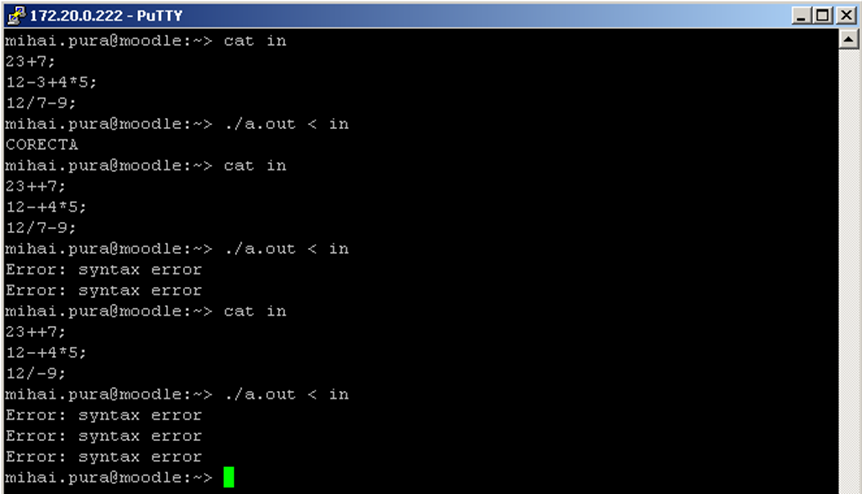
\includegraphics[width=\linewidth]{imgYacc20.png}
	\label{fig:schema20}
\end{figure}
\end{frame}



\begin{frame}{Depanarea}
\begin{itemize}
	\item
	Activarea pentru analizorul sintactic generat a facilităţilor de depanare oferite de de către yacc se face astfel:
	
	\begin{itemize}
		\item<cir@1->
		1. La crearea fişierului *.y, trebuie adăugată declaraţia:

		\item[]
		\hspace{2.9cm}{\color{red}int yydebug = 1;}

		\item[]
		în secţiunea de cod C a primei secţiuni a fişierului (adică între \%\{ şi \%\}).

		\item[]
		SAU

		\item[]
		\hspace{1cm}Se va folosi directiva {\color{red}\%debug}, în secţiunea de definiţii a primei secţiuni a fişierului

		\item<cir@1->
		2. La generarea fişierului sursă al analizorului sintactic, trebuie adăugate opţiunile {\color{red}--debug} şi {\color{red}--verbose}:

		\item[]
		\hspace{2.2cm}{\color{red}yacc –d *.y --debug --verbose}

	\end{itemize}


\end{itemize}
\end{frame}



\begin{frame}{Depanarea}
\begin{itemize}
	\item
	Aceste modificări vor duce la:

	\begin{itemize}
		\item<cir@1->
		1. Generarea fişierului {\color{red}y.output}, al cărui conţinut explică automatul finit implementat pentru analiza sintactică a gramaticii date.

		\item<cir@1->
		2. La rularea analizorului sintactic, se vor afişa informaţii cu privire la ceea ce se întâmplă în cadrul analizei.

	\end{itemize}

	\item
	La adresa:
	\newline

	\item[]
	\textbf{Debugging Lex, Yacc, etc.}
	
	\url{http://www.cs.man.ac.uk/~pjj/cs2121/debug.html}
	\newline
	
	se găsesc unele dintre cele mai obişnuite erori, precum şi modalităţile în care pot fi ele corectate.

\end{itemize}
\end{frame}



\begin{frame}
\begin{itemize}
\frametitle{Transmiterea informatiilor privind locatia atomilor lexicali}
\item
Analizorul lexical (yylex()) poate sa transmita analizorului sintactic informatii privind locatia atomilor lexicali în fisierul de intrare prin utilizarea variabilei \textcolor{red}{yylloc}.

\item
Aceasta este o variabila predefinita:

\item
\textcolor{red}{extern YYLTYPE yylloc;}

\item
yylloc poate fi accesata în codul asociat definitiei unui atom lexical si reprezinta informatiile de locatie pentru atomul lexical respectiv.

\item
YYLTYPE reprezinta o structure de date cu patru membri:
\item \color{red}
struct \{
\item
\quad int first\underline{ }line, last\underline{ }line;\\
\item
\quad int first\underline{ }column, last\underline{ }column;\\
\item
\};
\item \color{black}
yylex() trebuie deci sa completeze valoarea unora sau a tuturor membrilor variabilei yylloc cu valorile corespunzatoare calculate pe baza fisierului de intrare.

\end{itemize}
\end{frame}



\begin{frame}
\begin{itemize}
\frametitle{Transmiterea informatiilor privind locatia atomilor lexicali}
\item
Accesarea informatiilor privind locatia atomilor lexicali, se face în fisierul *.y în codul asociat partii drepte a unei reguli de productie prin utilizarea variabilelor \textcolor{red}{@i}, cu i de la 1 la numarul de elemente ale partii drepte a regulii de productie respective.
\item
Variabilele \textcolor{red}{@i} sunt de tipul YYLTYPE, la fel ca si variabila yylloc. În consecinta, ele au cei patru membrii ai structurii respective. 
\item
Bineînteles, se pot obtine valori numai pentru membrii structurii care au fost completati de catre yylex().
\item
În prima sectiune a fisierului *.y se va folosi directiva \textcolor{red}{\%locations}.

\end{itemize}
\end{frame}



\begin{frame}{Transmiterea valorii semantice a atomilor lexicali}
\begin{itemize}
	\item
	La fiecare apel al funcţiei yylex(), analizorul lexical returnează tipul următorului atom lexical, aşa cum au fost definiţi aceştia în fişierul *.y, prin \textbf{\%token}.

	\item
	Acest mecanism este suficient pentru analiza sintactică.

	\item
	În cazul în care se doreşte scrierea unui interpretor sau generarea de cod, pe lângă tipul atomilor lexicali este nevoie şi de valoarea acestora.

	\item
	În cele două exemple de până acum am scris un analizor sintactic pentru limbajul instrucţiunilor aritmetice. În cazul scrierii unui interpretor sau a generării de cod, pentru atomul lexical NUMAR este nevoie şi de valoarea acestuia, adică de valoarea numerică a succesiunii de caractere care s-a potrivit definiţiei acestuia.

\end{itemize}
\end{frame}



\begin{frame}{Transmiterea valorii semantice a atomilor lexicali}
\begin{itemize}
	\item
	În acest scop se poate utiliza variabila predefinită {\color{red}yylval}.

	\item
	Aceasta este declarată (în fişierul y.tab.c), în mod implicit, sub forma:
	
	\item[]
	\hspace{3cm}{\color{red}YYSTYPE yylval};

	\item
	În mod implicit, tipul de date YYSTYPE este definit în fişierul y.tab.c, ca fiind:
	
	\item[]
	\hspace{2.75cm}{\color{red}typedef int YYSTYPE};

	\item
	yylval reprezintă valoarea semantică a lookahead token-ului. 

	\item
	În fişierul *.l, în codul asociat definiţiei unui atom lexical, yylval poate fi utilizată pentru a transmite analizorului sintactic valoarea semantică a atomului lexical respectiv.

\end{itemize}
\end{frame}



\begin{frame}{Transmiterea valorii semantice a atomilor lexicali}
\begin{itemize}
	\item
	Pentru a utiliza variabile de tip {\color{red}struct} sau {\color{red}class} in interiorul lui {\color{red}\%union}, putem utiliza una dintre cele două variante de mai jos:

	\begin{itemize}
		\item<cir@1->
		1. se declară structura sau clasa chiar in {\color{red}interiorul lui \%union}:
			\linebreak

		\item[]
		\%union {int a; struct Exemplu {int a;char b;} Ex; }
			\linebreak

		\item<cir@1->
		2. folosim {\color{red}\%code requires}   inainte de {\color{red}\%union}:
			\linebreak

		\item[]
		\%code requires

		\item[]
		\{

		\begin{itemize}
			\item[]
			typedef struct exemplu {int a; char b;}	\hspace{1cm}EXEMPLU;
		\end{itemize}

		\item[]
		\}

		\item[]
		\%union {int a; EXEMPLU x; }
			\linebreak

		\item<cir@1->
		3. includem definiţia intr-un fişier header pe care îl includem in .l înainte de orice şi cumva la fel si in .y.

	\end{itemize}

\end{itemize}
\end{frame}



\begin{frame}{Transmiterea valorii semantice a atomilor lexicali}
\begin{itemize}
	\item
	În fişierul *.y, în codul asociat părţii drepte a unei reguli de producţie, se poate accesa valoarea semantică a atomilor lexicali sau a neterminalelor prin utilizarea variabilelor {\color{red}\$i}, cu i de la 1 la numărul de elemente ale părţii drepte a regulii de producţie respective.

	\item
	Analog, {\color{red}\$\$} reprezintă valoarea semantică care va asociată noului neterminal din vârful stivei, după ce are loc reducerea acestuia conform regulii de producţie respective.

	\item
	În mod implicit, yacc/bison consideră neterminalele şi atomii lexicali ca având o valoarea semantică de tip {\color{red}int}.

\end{itemize}
\end{frame}



\begin{frame}{Ex3 din arhiva - Transmiterea valorii semantice a atomilor lexicali}
\begin{itemize}
	\item[]
	\footnotesize\%\{
	
	\begin{itemize}
		\item[]
		\#include "y.tab.h"

		\item[]
		extern int yylval;

		\item[]
		int lineNo = 1;

		\item[]
		int colNo = 1;
	\end{itemize}
	
	\item[]
	\footnotesize\%\}

	\item[]
	\footnotesize\%\%

	\item[]
	"+" \hspace{1.55cm} \{ colNo++; return TOK\_PLUS; \}

	\item[]
	"-" \hspace{1.7cm} \{ colNo++; return TOK\_MINUS; \}

	\item[]
	"*" \hspace{1.65cm} \{ colNo++; return TOK\_MULTIPLY; \}

	\item[]
	"/" \hspace{1.65cm} \{ colNo++; return TOK\_DIVIDE; \}

	\item[]
	"(" \hspace{1.7cm} \{ colNo++; return TOK\_LEFT; \}

	\item[]
	")" \hspace{1.7cm} \{ colNo++; return TOK\_RIGHT; \}

	\item[]
	";" \hspace{1.75cm} \{ colNo++; return ';'; \}

	\item[]
	0|[1-9][0-9]* \hspace{0.5cm} \{ colNo+=strlen(yytext); yylloc.first\_line = lineNo; yylloc.first\_column = colNo; {\color{red}yylval = atoi(yytext)}; return TOK\_NUMBER;  \}

	\item[]
	. \hspace{2cm} \{ colNo++; return TOK\_ERROR; \}

	\item[]
	\textbackslash n \hspace{1.95cm}\{ lineNo++;colNo=1;  \}

	\item[]
	\footnotesize\%\%

\end{itemize}
\end{frame}



\begin{frame}{Ex3 din arhiva}
\begin{itemize}
\item[]
	\%\{
	
	\begin{itemize}
		\item[]
		\#include <stdio.h>
		
		\item[]
		int EsteCorecta = 1;

		\item[]
		char msg[50];

	\end{itemize}
	
	\item[]
	\%\}
		\linebreak

	\item[]
	\%token TOK\_PLUS TOK\_MINUS TOK\_MULTIPLY TOK\_DIVIDE TOK\_LEFT TOK\_RIGHT TOK\_ERROR

	\item[]
	\%token TOK\_NUMBER
		\linebreak

	\item[]
	\%start S
		\linebreak

	\item[]
	\%left TOK\_PLUS TOK\_MINUS

	\item[]
	\%left TOK\_MULTIPLY TOK\_DIVIDE


\end{itemize}
\end{frame}



\begin{frame}{Ex3 din arhiva}
\begin{itemize}
	\item[]
	 \%\%
	
	\item[]
	S :
	
	\begin{itemize}
		\item[]
		|

		\item[]
		E ';' S \{ printf("= \%d \textbackslash n", \$1); \}
		
		\item[]
		|

		\item[]
		error ';' S
		
		\item[]
		\hspace{0.5cm}\{ EsteCorecta = 0;\}

		\item[]
		;
	\end{itemize}

\end{itemize}
\end{frame}



\begin{frame}{Ex3 din arhiva}
\begin{itemize}
	\item[]
		\scriptsize E : E TOK\_PLUS E \{ \$\$ = \$1 + \$3; \}
	
			\begin{itemize}
				\item[]
				 \scriptsize |
	
				\item[]
				 \scriptsize E TOK\_MINUS E \{ \$\$ = \$1 - \$3; \}
	
				\item[]
				\scriptsize |
	
				\item[]
				\scriptsize E TOK\_MULTIPLY E \{ \$\$ = \$1 * \$3; \}
	
				\item[]
				\scriptsize |
	
				\item[]
				\scriptsize E TOK\_DIVIDE E
				
				\begin{itemize}
					\item[]
					\scriptsize \{
						
					\item[]
					\hspace{0.5cm}if(\$3 == 0) 
						
					\item[]
					\hspace{0.5cm}\{

					\item[]
					\hspace{1cm}sprintf(msg,"\%d:\%d Eroare semantica: Impartire la zero!", @1.first\_line, @1.first\_column);

					\item[]
					\hspace{1cm}yyerror(msg);

					\item[]
					\hspace{1cm}YYERROR;
		
					\item[]
					\hspace{0.5cm}\}
		
					\item[]
					\hspace{0.5cm}else \{ \$\$ = \$1 / \$3; \} 

					\item[]
					\}
				\end{itemize}
	
				\item[]
				\scriptsize |
	
				\item[]
				\scriptsize TOK\_LEFT E TOK\_RIGHT \{ \$\$ = \$2; \}
	
				\item[]
				\scriptsize |
	
				\item[]
				\scriptsize TOK\_NUMBER \{ \$\$ = \$1; \}
	
				\item[]
				      ;
			\end{itemize}
	
		\item[]
		\scriptsize
 \%\%

\end{itemize}
\end{frame}



\begin{frame}{Ex3 din arhiva}
\begin{itemize}
	\item[]
	int main()

	\item[]
	\{

		\begin{itemize}
			\item[]
			yyparse();
				\linebreak

			\item[]
			if(EsteCorecta == 1)

			\item[]
			\{
				
				\begin{itemize}
					\item[]
					printf("CORECTA \textbackslash n");
				\end{itemize}

			\item[]
			\}
				\linebreak

			\item[]
			return 0;
		\end{itemize}

	\item[]
	\}
		\linebreak

	\item[]
	int yyerror(const char *msg)

	\item[]
	\{

		\begin{itemize}
			\item[]
			printf("Error: \%s \textbackslash n", msg);

			\item[]
			return 1;
		\end{itemize}

	\item[]
	\}

\end{itemize}
\end{frame}



\begin{frame}{Transmiterea valorii semantice a atomilor lexicali}
\begin{columns}
\begin{column}{0.5\textwidth}
\begin{itemize}
	\item
	E $\rightarrow$ E + E

	\item
	E $\rightarrow$ E - E

	\item
	E $\rightarrow$ E * E

	\item
	E $\rightarrow$ E / E

	\item
	E $\rightarrow$ (E)

	\item
	E $\rightarrow$ NR

\end{itemize}
\end{column}

\begin{column}{0.4\textwidth}

\begin{tabular}{ccc|} \cline{1-3}
\multicolumn{1}{|c}{\textbf{Intrare}} & {1+2} & {\textbf{yylval}} \\ \cline{1-3}
\multicolumn{1}{|c}{\textbf{Lookahead}} & $\varepsilon$ & $\varepsilon$ \\ \cline{1-3} \\
\end{tabular}
\begin{tabular}{cc|c|}
\cline{1-1}
\multicolumn{1}{|c|}{\textbf{Stiva}} & \hspace{0.75cm}\\
\multicolumn{1}{|c|}{$\varepsilon$} & \hspace{0.75cm}\\
\cline{1-1}
\end{tabular}

\end{column}
\end{columns}
\end{frame}



\begin{frame}{Transmiterea valorii semantice a atomilor lexicali}
\begin{columns}
\begin{column}{0.5\textwidth}
\begin{itemize}
	\item
	E $\rightarrow$ E + E

	\item
	E $\rightarrow$ E - E

	\item
	E $\rightarrow$ E * E

	\item
	E $\rightarrow$ E / E

	\item
	E $\rightarrow$ (E)

	\item
	E $\rightarrow$ NR

\end{itemize}
\end{column}

\begin{column}{0.4\textwidth}

\begin{tabular}{ccc|} \cline{1-3}
\multicolumn{1}{|c}{\textbf{Intrare}} & {1+2} & {\textbf{yylval}} \\ \cline{1-3}
\multicolumn{1}{|c}{\textbf{Lookahead}} & NR & 1 \\ \cline{1-3} \\
\end{tabular}
\begin{tabular}{cc|c|}
\cline{1-1}
\multicolumn{1}{|c|}{\textbf{Stiva}} & \hspace{0.75cm}\\
\multicolumn{1}{|c|}{$\varepsilon$} & \hspace{0.75cm}\\
\cline{1-1}
\end{tabular}

\end{column}
\end{columns}
\end{frame}



\begin{frame}{Transmiterea valorii semantice a atomilor lexicali}
\begin{columns}
\begin{column}{0.5\textwidth}
\begin{itemize}
	\item
	E $\rightarrow$ E + E

	\item
	E $\rightarrow$ E - E

	\item
	E $\rightarrow$ E * E

	\item
	E $\rightarrow$ E / E

	\item
	E $\rightarrow$ (E)

	\item
	E $\rightarrow$ NR

\end{itemize}
\end{column}

\begin{column}{0.4\textwidth}

\begin{tabular}{ccc|} \cline{1-3}
\multicolumn{1}{|c}{\textbf{Intrare}} & {1+2} & {\textbf{yylval}} \\ \cline{1-3}
\multicolumn{1}{|c}{\textbf{Lookahead}} & + & $\varepsilon$ \\ \cline{1-3} \\
\end{tabular}
\begin{tabular}{cc|c|}
\cline{1-1}
\multicolumn{1}{|c|}{\textbf{Stiva}} & \hspace{0.75cm}\\
\multicolumn{1}{|c|}{NR} & \hspace{0.75cm} & (\$1 = 1)\\
\cline{1-1}
\end{tabular}

\end{column}
\end{columns}
\end{frame}



\begin{frame}{Transmiterea valorii semantice a atomilor lexicali}
\begin{columns}
\begin{column}{0.5\textwidth}
\begin{itemize}
	\item
	E $\rightarrow$ E + E

	\item
	E $\rightarrow$ E - E

	\item
	E $\rightarrow$ E * E

	\item
	E $\rightarrow$ E / E

	\item
	E $\rightarrow$ (E)

	\item
	E $\rightarrow$ NR

\end{itemize}
\end{column}

\begin{column}{0.4\textwidth}

\begin{tabular}{ccc|} \cline{1-3}
\multicolumn{1}{|c}{\textbf{Intrare}} & {1+2} & {\textbf{yylval}} \\ \cline{1-3}
\multicolumn{1}{|c}{\textbf{Lookahead}} & + & $\varepsilon$ \\ \cline{1-3} \\
\end{tabular}
\begin{tabular}{cc|c|}
\cline{1-1}
\multicolumn{1}{|c|}{\textbf{Stiva}} & \hspace{0.75cm}\\
\multicolumn{1}{|c|}{E} & \hspace{0.75cm} & \$\$ = \$1\\
\cline{1-1}
\end{tabular}

\end{column}
\end{columns}
\end{frame}



\begin{frame}{Transmiterea valorii semantice a atomilor lexicali}
\begin{columns}
\begin{column}{0.5\textwidth}
\begin{itemize}
	\item
	E $\rightarrow$ E + E

	\item
	E $\rightarrow$ E - E

	\item
	E $\rightarrow$ E * E

	\item
	E $\rightarrow$ E / E

	\item
	E $\rightarrow$ (E)

	\item
	E $\rightarrow$ NR

\end{itemize}
\end{column}

\begin{column}{0.4\textwidth}

\begin{tabular}{ccc|} \cline{1-3}
\multicolumn{1}{|c}{\textbf{Intrare}} & {1+2} & {\textbf{yylval}} \\ \cline{1-3}
\multicolumn{1}{|c}{\textbf{Lookahead}} & NR & 2 \\ \cline{1-3} \\
\end{tabular}
\begin{tabular}{cc|c|}
\cline{1-1}
\multicolumn{1}{|c|}{\textbf{Stiva}} & \hspace{0.75cm}\\
\multicolumn{1}{|c|} {+}  & \hspace{0.75cm}\\
\multicolumn{1}{|c|}{E} & \hspace{0.75cm} & (\$2 = 1)\\
\cline{1-1}
\end{tabular}

\end{column}
\end{columns}
\end{frame}



\begin{frame}{Transmiterea valorii semantice a atomilor lexicali}
\begin{columns}
\begin{column}{0.5\textwidth}
\begin{itemize}
	\item
	E $\rightarrow$ E + E

	\item
	E $\rightarrow$ E - E

	\item
	E $\rightarrow$ E * E

	\item
	E $\rightarrow$ E / E

	\item
	E $\rightarrow$ (E)

	\item
	E $\rightarrow$ NR

\end{itemize}
\end{column}

\begin{column}{0.4\textwidth}

\begin{tabular}{ccc|} \cline{1-3}
\multicolumn{1}{|c}{\textbf{Intrare}} & {1+2} & {\textbf{yylval}} \\ \cline{1-3}
\multicolumn{1}{|c}{\textbf{Lookahead}} & $\varepsilon$ & $\varepsilon$ \\ \cline{1-3} \\
\end{tabular}
\begin{tabular}{cc|c|}
\cline{1-1}
\multicolumn{1}{|c|}{\textbf{Stiva}} & \hspace{0.75cm}\\
\multicolumn{1}{|c|} {NR}  & \hspace{0.75cm} & (\$1 = 2)\\
\multicolumn{1}{|c|} {+}  & \hspace{0.75cm}\\
\multicolumn{1}{|c|}{E} & \hspace{0.75cm} & (\$3 = 1)\\
\cline{1-1}
\end{tabular}

\end{column}
\end{columns}
\end{frame}



\begin{frame}{Transmiterea valorii semantice a atomilor lexicali}
\begin{columns}
\begin{column}{0.5\textwidth}
\begin{itemize}
	\item
	E $\rightarrow$ E + E

	\item
	E $\rightarrow$ E - E

	\item
	E $\rightarrow$ E * E

	\item
	E $\rightarrow$ E / E

	\item
	E $\rightarrow$ (E)

	\item
	E $\rightarrow$ NR

\end{itemize}
\end{column}

\begin{column}{0.4\textwidth}

\begin{tabular}{ccc|} \cline{1-3}
\multicolumn{1}{|c}{\textbf{Intrare}} & {1+2} & {\textbf{yylval}} \\ \cline{1-3}
\multicolumn{1}{|c}{\textbf{Lookahead}} & $\varepsilon$ & $\varepsilon$ \\ \cline{1-3} \\
\end{tabular}
\begin{tabular}{cc|c|}
\cline{1-1}
\multicolumn{1}{|c|}{\textbf{Stiva}} & \hspace{0.75cm}\\
\multicolumn{1}{|c|} {E}  & \hspace{0.75cm} & \$\$ = \$1\\
\multicolumn{1}{|c|} {+}  & \hspace{0.75cm}\\
\multicolumn{1}{|c|}{E} & \hspace{0.75cm} & (\$3 = 1)\\
\cline{1-1}
\end{tabular}

\end{column}
\end{columns}
\end{frame}



\begin{frame}{Transmiterea valorii semantice a atomilor lexicali}
\begin{columns}
\begin{column}{0.5\textwidth}
\begin{itemize}
	\item
	E $\rightarrow$ E + E

	\item
	E $\rightarrow$ E - E

	\item
	E $\rightarrow$ E * E

	\item
	E $\rightarrow$ E / E

	\item
	E $\rightarrow$ (E)

	\item
	E $\rightarrow$ NR

\end{itemize}
\end{column}

\begin{column}{0.4\textwidth}

\begin{tabular}{ccc|} \cline{1-3}
\multicolumn{1}{|c}{\textbf{Intrare}} & {1+2} & {\textbf{yylval}} \\ \cline{1-3}
\multicolumn{1}{|c}{\textbf{Lookahead}} & $\varepsilon$ & $\varepsilon$ \\ \cline{1-3} \\
\end{tabular}
\begin{tabular}{cc|c|}
\cline{1-1}
\multicolumn{1}{|c|}{\textbf{Stiva}} & \hspace{0.75cm}\\
\multicolumn{1}{|c|} {E}  & \hspace{0.75cm} & (\$1 = 2)\\
\multicolumn{1}{|c|} {+}  & \hspace{0.75cm}\\
\multicolumn{1}{|c|}{E} & \hspace{0.75cm} & (\$3 = 1)\\
\cline{1-1}
\end{tabular}

\end{column}
\end{columns}
\end{frame}



\begin{frame}{Transmiterea valorii semantice a atomilor lexicali}
\begin{columns}
\begin{column}{0.5\textwidth}
\begin{itemize}
	\item
	E $\rightarrow$ E + E

	\item
	E $\rightarrow$ E - E

	\item
	E $\rightarrow$ E * E

	\item
	E $\rightarrow$ E / E

	\item
	E $\rightarrow$ (E)

	\item
	E $\rightarrow$ NR

\end{itemize}
\end{column}

\begin{column}{0.4\textwidth}

\begin{tabular}{ccc|} \cline{1-3}
\multicolumn{1}{|c}{\textbf{Intrare}} & {1+2} & {\textbf{yylval}} \\ \cline{1-3}
\multicolumn{1}{|c}{\textbf{Lookahead}} & $\varepsilon$ & $\varepsilon$ \\ \cline{1-3} \\
\end{tabular}
\begin{tabular}{cc|c|}
\cline{1-1}
\multicolumn{1}{|c|}{\textbf{Stiva}} & \hspace{0.75cm}\\
\multicolumn{1}{|c|} {E}  & \hspace{0.75cm} & \$\$ = \$1 + \$3\\
\cline{1-1}
\end{tabular}

\end{column}
\end{columns}
\end{frame}



\begin{frame}
\begin{itemize}
\frametitle{Transmiterea valorii semantice a atomilor lexicali}
\item
La scrierea unui interpretor sau a unui compilator pentru un limbaj complex, este insuficient mecanismul de transmitere a valorilor atomilor lexicali prin variabile yylval de tip YYSTYPE de tip întreg.
\item
Atunci când atomii lexicali ai limbajului au tipuri de valori semantice diferite, YYSTYPE poate fi definit de tipul \textcolor{red}{union}, astfel încât variabila yylval sa aiba un membru special, corespunzatorul tipului fiecaruia dintre atomii lexicali.
\item
Declararea acesteia se face în fisierul *.y, prin:
\item
\quad \textcolor{red}{\%union \{ membrii structurii de tip union ... \}}

\end{itemize}
\end{frame}



\begin{frame}
\begin{itemize}
\frametitle{Transmiterea valorii semantice a atomilor lexicali}
\item
Ca urmare a acestei declaratii, header-ul y.tab.h va contine definitia corespunzatoare a tipului de date YYSTYPE:
\item \color{red}
typedef union \{
\item \qquad
membrii structurii de tip union ... 
\item \qquad
\} YYSTYPE;
\item \color{black}
Dupa declararea uniunii, trebuie asociat fiecarui atom lexical cu valoarea semantica, câte un membru al acesteia.
\item
Referirea unui membru al uniunii în fisierul *.y se face prin constructia:
\item \qquad
\textcolor{red}{<num\underline{ }membru\underline{ }uniune>}

\end{itemize}
\end{frame}



\begin{frame}
\begin{itemize}
\frametitle{Transmiterea valorii semantice a atomilor lexicali}
\item
Asocierea dintre un membru al uniunii si un atom lexical se poate face prin una din declaratiile \textcolor{red}{\%token}, \textcolor{red}{\%left}, \textcolor{red}{\%right} si \textcolor{red}{\%nonassoc}.
\item \vspace{5mm}
\%token <nume\underline{ }membru> lista nume atomi lexicali
\item
\%left <nume\underline{ }membru> lista nume atomi lexicali
\item
\%right <nume\underline{ }membru> lista nume atomi lexicali
\item
\%nonassoc <nume\underline{ }membru> lista nume atomi lexicali

\end{itemize}
\end{frame}



\begin{frame}
\begin{itemize}
\frametitle{Transmiterea valorii semantice a atomilor lexicali}
\item
Analog, se va utiliza declaratia \textcolor{red}{\%type} pentru a asocia un membru al uniunii, unui neterminal.
\item \vspace{5mm}
\%type <nume\underline{ }membru> lista neterminale
\item \vspace{5mm}
Acest lucru este necesar pentru codul asociat partii drepte a unei reguli de productie, în care se da o valoarea semantica noului vârf al stivei, cel rezultat în urma reducerii conform regulii de productie respective.

\end{itemize}
\end{frame}



\begin{frame}
\begin{itemize}
\frametitle{Transmiterea valorii semantice a atomilor lexicali}
\item
În cazurile în care mecanismul descris este insuficient, se poate preciza “pe loc” tipul valorii semantice a unui atom lexical sau a unui neterminal.
\item
Acest lucru se face inserând dupa primul \$ numele membrului uniunii (între <>), care va fi asociat elementului respectiv (atom lexical sau neterminal).
\item
\textcolor{red}{\$<nume\underline{ }membru>\$}
\item
\textcolor{red}{\$<nume\underline{ }membru>|}
\item \vspace{5mm}
Ex:
\item
rule : aaa \{ \$<intval>\$ = 3; \}
\item \qquad
|
\item \qquad
bbb \{ fun( \$<intval>2,\$<other>0 ); \} 
\item \qquad
;
\item \vspace{5mm}
Obs: \$0 reprezinta valorile contextului stânga.

\end{itemize}
\end{frame}



\begin{frame}
\begin{itemize}
\frametitle{Transmiterea valorii semantice a atomilor lexicali}
\item
Membrii structurii de tip union declarate pot fi si variabile de tip \textcolor{red}{struct/class}, daca acest lucru este necesar.
\item \vspace{5mm}
Ex:
\item \vspace{5mm}
\%\{
\item
// ...
\item
\textcolor{red}{typedef struct interval \{ double lo, hi; \} INTERVAL;}
\item
\%\}
\item
...
\item
\%union \{ int ival; double dval; \textcolor{red}{INTERVAL vval;} \} 

\end{itemize}
\end{frame}



\begin{frame}
\begin{itemize}
\frametitle{Analiza semantica}
\item
Analiza semantica se face în paralel cu analiza sintactica.
\item
Ea depinde de limbajul tinta al interpretorului/compilatorului.
\item
Daca la analiza semantica se constata erori, interpretarea, sau respectiv generarea codului trebuie întrerupta.
\item
Analiza sintactica si cea semantica trebuie însa se continue, pentru a gasi si afisa toate eventualele erori.
\end{itemize}
\end{frame}



\begin{frame}{Ex4 din arhiva - Analiza semantica}
\begin{itemize}
\item
\%\{
\item \qquad
\#include "y.tab.h"
\item \qquad
int lineNo = 1;
\item \qquad
int colNo = 1;
\item
\%\}
\item \vspace{5mm}
\%\%
\item
"+"\hspace{20mm}\{ colNo++; return TOK\underline{ }PLUS; \}
\item
"-"\hspace{21.7mm}\{ colNo++; return TOK\underline{ }MINUS; \}
\item
"*"\hspace{21mm}\{ colNo++; return TOK\underline{ }MULTIPLY; \}
\item
"/"\hspace{21mm}\{ colNo++; return TOK\underline{ }DIVIDE; \}
\item
"("\hspace{21.5mm}\{ colNo++; return TOK\underline{ }LEFT; \}
\item
")"\hspace{21.5mm}\{ colNo++; return TOK\underline{ }RIGHT; \}
\item
";"\hspace{22mm}\{ colNo++; return ';'; \}
\item
"="\hspace{20mm}\{ colNo++; return '='; \}
\end{itemize}
\end{frame}



\begin{frame}{Ex4 din arhiva}
\begin{itemize}
\item
0|[1-9][0-9]*\hspace{7.5mm}\{ 
\begin{itemize}
\item
yylloc.first\underline{ }line = lineNo; 
\item
yylloc.first\underline{ }column = colNo; 
\item
colNo+=strlen(yytext);
\item
yylval.val = atoi(yytext);
\item
return TOK\underline{ }NUMBER; \}
\end{itemize}
\item
"var“\hspace{19mm}\{ colNo+=3; return TOK\underline{ }DECLARE; \}
\item
"print“\hspace{16.2mm}\{ colNo+=5; return TOK\underline{ }PRINT; \}
\item
\text{[a-zA-Z][a-zA-Z0-9]*} \{ 
\begin{itemize}
\item
yylloc.first\underline{ }line = lineNo;
\item
yylloc.first\underline{ }column = colNo; 
\item
colNo+=strlen(yytext); 
\item
yylval.sir = new char[strlen(yytext)+1];
\item 
strcpy(yylval.sir,yytext); 
\item
return TOK\underline{ }VARIABLE;\}
\end{itemize}
\item
\text{[ ]}\hspace{24.5mm}\{ colNo++; \} 
\item
.\hspace{26.5mm}\{ colNo++; return TOK\underline{ }ERROR; \}
\item
\textbackslash{n}\hspace{24mm}\{ lineNo++;colNo=1; \}
\item
\%\%

\end{itemize}
\end{frame}



\begin{frame}{Ex4 din arhiva}
\begin{itemize}
\item
\%\{
\item \qquad
\#include <stdio.h>
\item \qquad
\#include <string.h>
\item \qquad \vspace{5mm}
int yylex();
\item \qquad
int yyerror(const char *msg);
\item \qquad \vspace{5mm}
int EsteCorecta = 1;
\item \qquad
char msg[50];

\end{itemize}
\end{frame}



\begin{frame}{Ex4 din arhiva}
\begin{itemize}
\item
class TVAR
\item \hspace{4mm}
\{
\item \qquad
char* nume;
\item \qquad
int valoare;
\item \qquad
TVAR* next;
\item \hspace{4mm} \vspace{5mm}
public:
\item \qquad
static TVAR* head;
\item \qquad \vspace{5mm}
static TVAR* tail;
\item \qquad 
TVAR(char* n, int v = -1);
\item \qquad
TVAR();
\item \qquad
int exists(char* n);
\item \qquad
void add(char* n, int v = -1);
\item \qquad
int getValue(char* n);
\item \qquad
void setValue(char* n, int v);
\item \hspace{4mm}
\};

\end{itemize}
\end{frame}



\begin{frame}{Ex4 din arhiva}
\begin{itemize}
\item
TVAR* TVAR::head;
\item \hspace{4mm}
TVAR* TVAR::tail;
\item \vspace{6mm} \hspace{4mm}
TVAR::TVAR(char* n, int v)
\item \hspace{4mm}
\{
\item \hspace{6mm}
this->nume = new char[strlen(n)+1];
\item \hspace{6mm}
strcpy(this->nume,n);
\item \hspace{6mm}
this->valoare = v;
\item \hspace{5mm}
this->next = NULL;
\item \hspace{4mm}
\}
\item \vspace{6mm} \hspace{4mm}
TVAR::TVAR()
\item \hspace{4mm}
\{
\item \hspace{6mm}
TVAR::head = NULL;
\item \hspace{6mm}
TVAR::tail = NULL;
\item \hspace{4mm}
\}

\end{itemize}
\end{frame}



\begin{frame}{Ex4 din arhiva}
\begin{itemize}
\item
int TVAR::exists(char* n)
\item \hspace{4mm}
	\{
\item \hspace{6mm}
	  TVAR* tmp = TVAR::head;
\item \hspace{6mm}
	  while(tmp != NULL)
\item \hspace{6mm}
	  \{
\item \hspace{8mm}  
	    if(strcmp(tmp->nume,n) == 0)
\item \hspace{10mm}
	      return 1;
\item \hspace{10mm}
          tmp = tmp->next;
\item \hspace{6mm}         
	  \}
\item \hspace{6mm}
	  return 0;
\item \hspace{4mm}
	 \}

\end{itemize}
\end{frame}



\begin{frame}{Ex4 din arhiva}
\begin{itemize}
\item
void TVAR::add(char* n, int v)
\item \hspace{4mm}
	 \{
\item \hspace{6mm}
	   TVAR* elem = new TVAR(n, v);
\item \hspace{6mm}
	   if(head == NULL)
\item \hspace{6mm}
	   \{
\item \hspace{8mm}
	     TVAR::head = TVAR::tail = elem;
\item \hspace{6mm}
	   \}
\item \hspace{6mm}
	   else
\item \hspace{6mm}
	   \{
\item \hspace{8mm}
	     TVAR::tail->next = elem;
\item \hspace{8mm}
	     TVAR::tail = elem;
\item \hspace{6mm}	     
	   \}
\item \hspace{4mm}
	 \}
\end{itemize}
\end{frame}



\begin{frame}{Ex4 din arhiva}
\begin{itemize}
\item
 int TVAR::getValue(char* n)
\item \hspace{4mm}
	 \{
\item \hspace{6mm}
	   TVAR* tmp = TVAR::head;
\item \hspace{6mm}
	   while(tmp != NULL)
\item \hspace{6mm}
	   \{
\item \hspace{8mm}
	     if(strcmp(tmp->nume,n) == 0)
\item \hspace{10mm}
	      return tmp->valoare;
\item \hspace{8mm}
	     tmp = tmp->next;
\item \hspace{6mm}
	   \}
\item \hspace{6mm}
	   return -1;
\item \hspace{4mm}
	  \}
\end{itemize}
\end{frame}



\begin{frame}{Ex4 din arhiva}
\begin{itemize}
\item \hspace{4mm}
	  void TVAR::setValue(char* n, int v)
\item \hspace{4mm}
	  \{
\item \hspace{6mm}
	    TVAR* tmp = TVAR::head;
\item \hspace{6mm}
	    while(tmp != NULL)
\item \hspace{6mm}
	    \{
\item \hspace{8mm}
	      if(strcmp(tmp->nume,n) == 0)
\item \hspace{8mm}
	      \{
\item \hspace{12mm}
		tmp->valoare = v;
\item \hspace{8mm}
	      \}
\item \hspace{8mm}
	      tmp = tmp->next;
\item \hspace{6mm}
	    \}
\item \hspace{4mm} 
	  \}
\item \hspace{2mm}
	TVAR* ts = NULL;
\%\}
\end{itemize}
\end{frame}



\begin{frame}{Ex4 din arhiva}
\begin{itemize}
\item 
\%union \{ char* sir; int val; \}
\item \vspace{4mm}
\%token TOK\underline{ }PLUS TOK\underline{ }MINUS TOK\underline{ }MULTIPLY TOK\underline{ }DIVIDE TOK\underline{ }LEFT TOK\underline{ }RIGHT TOK\underline{ }DECLARE TOK\underline{ }PRINT
\item
\%token <val> TOK\underline{ }NUMBER
\item
\%token <sir> TOK\underline{ }VARIABLE
\item \vspace{5mm}
\%type <val> E
\item \vspace{4mm}
\%start S
\item \vspace{4mm}
\%left TOK\underline{ }PLUS TOK\underline{ }MINUS
\item
\%left TOK\underline{ }MULTIPLY TOK\underline{ }DIVIDE
\item \vspace{4mm}
\%locations
\item \vspace{4mm}
\%\%

\end{itemize}
\end{frame}



\begin{frame}{Ex4 din arhiva}
\begin{itemize}
\item 
S : 
\item \hspace{4mm} 
    |
\item \hspace{4mm} 
    I ';' S
\item \hspace{4mm} 
    | 
\item \hspace{4mm} 
    error ';' S
\item \hspace{6mm} 
       \{ EsteCorecta = 0; \}
\item \hspace{4mm} 
    ;
\end{itemize}
\end{frame}



\begin{frame}{Ex4 din arhiva}
\begin{itemize}
\item
I : TOK\underline{ }VARIABLE '=' E
\item \hspace{4mm}
      \{
\item \hspace{6mm}
	if(ts != NULL)
\item \hspace{6mm}
	\{
\item \hspace{8mm}
	  if(ts->exists(\$1) == 1)
\item \hspace{8mm}
	  \{
\item \hspace{10mm}
	    ts->setValue(\$1, \$3);
\item \hspace{8mm}
	  \}
\item \hspace{8mm}
	  else
\item \hspace{8mm}
	  \{
\item \hspace{10mm}
	    sprintf(msg,"\%d:\%d Eroare semantica: Variabila \%s este utilizata fara sa fi fost declarata!", @1.first\underline{ }line, @1.first\underline{ }column, \$1);
\item \hspace{10mm}
	    yyerror(msg);
\item \hspace{10mm}
	    YYERROR;
\item \hspace{8mm}
	  \}
\item \hspace{6mm}
	\}
\end{itemize}
\end{frame}



\begin{frame}{Ex4 din arhiva}
\begin{itemize}
\item
else
\item \hspace{4mm}
\{
\item \hspace{6mm}
	  sprintf(msg,"\%d:\%d Eroare semantica: Variabila \%s este utilizata fara sa fi fost declarata!", @1.first\underline{ }line, @1.first\underline{ }column, \$1);
\item \hspace{6mm}
	  yyerror(msg);
\item \hspace{6mm}
	  YYERROR;
\item \hspace{4mm}
	\}
\item \hspace{5mm}	
      \}
\item \hspace{4mm}
    |
\end{itemize}
\end{frame}



\begin{frame}[shrink=20]{Ex4 din arhiva}
\begin{itemize}
\item
 TOK\underline{ }DECLARE TOK\underline{ }VARIABLE
\item \hspace{4mm}
      \{
\item \hspace{6mm}
	if(ts != NULL)
\item \hspace{6mm}
	\{
\item \hspace{8mm}
	  if(ts->exists(\$2) == 0)
\item \hspace{8mm}
	  \{
\item \hspace{10mm}
	    ts->add(\$2);
\item \hspace{8mm}
	  \}
\item \hspace{8mm}
	  else
\item \hspace{8mm}
	  \{
\item \hspace{10mm}
	    sprintf(msg,"\%d:\%d Eroare semantica: Declaratii multiple pentru variabila \%s!", @1.first\underline{ }line, @1.first\underline{ }column, \$2);
\item \hspace{10mm}
	    yyerror(msg);
\item \hspace{10mm}
	    YYERROR;
\item \hspace{8mm}
	  \}
\item \hspace{6mm}
	\}
\item \hspace{6mm}
	else
\item \hspace{6mm}
	\{
\item \hspace{8mm}
	  ts = new TVAR();
\item \hspace{8mm}
	  ts->add(\$2);
\item \hspace{6mm}
	\}
\item \hspace{4mm}
      \}
\item \hspace{2mm}
    |
\end{itemize}
\end{frame}



\begin{frame}{Ex4 din arhiva}
\begin{itemize}
\item \hspace{4mm}
 TOK\underline{ }PRINT TOK\underline{ }VARIABLE
      \{
\item \hspace{6mm}
	if(ts != NULL)
\item \hspace{6mm}
	\{
\item \hspace{6mm}
	  if(ts->exists(\$2) == 1)
\item \hspace{6mm}
	  \{
\item \hspace{8mm}
	    if(ts->getValue(\$2) == -1)
\item \hspace{8mm}
	    \{
\item \hspace{10mm}
	      sprintf(msg,"\%d:\%d Eroare semantica: Variabila \%s este utilizata fara sa fi fost initializata!", @1.first\underline{ }line, @1.first\underline{ }column, \$2);
\item \hspace{10mm}	      
	      yyerror(msg);
\item \hspace{10mm}
	      YYERROR;
\item \hspace{8mm}
	    \}
\item \hspace{8mm}
	    else
\item \hspace{8mm}
	    \{
\item \hspace{10mm}
	      printf("\%d",ts->getValue(\$2));
\item \hspace{8mm}	      
	    \}
\item \hspace{6mm}
	  \}
\end{itemize}
\end{frame}



\begin{frame}[shrink=10]{Ex4 din arhiva}
\begin{itemize}
\item 
 else
 \item \hspace{4mm}
	  \{
\item \hspace{6mm}
	    sprintf(msg,"\%d:\%d Eroare semantica: Variabila \%s este utilizata fara sa fi fost declarata!", @1.first\underline{ }line, @1.first\underline{ }column, \$2);
\item \hspace{6mm}
	    yyerror(msg);
\item \hspace{6mm}
	    YYERROR;
\item \hspace{4mm}
	  \}
\item \hspace{3mm}
	\}
\item \hspace{3mm}
	else
\item \hspace{3mm}
	\{
\item \hspace{4mm}
	  sprintf(msg,"\%d:\%d Eroare semantica: Variabila \%s este utilizata fara sa fi fost declarata!", @1.first\underline{ }line, @1.first\underline{ }column, \$2);
\item \hspace{4mm}
	  yyerror(msg);
\item \hspace{4mm}
	  YYERROR;
\item \hspace{3mm}
	\}
\item \hspace{2mm}
      \}
\item \hspace{1mm}
    ;
\end{itemize}
\end{frame}



\begin{frame}{Ex4 din arhiva}
\begin{itemize}
\item
E : E TOK\underline{ }PLUS E \{ \$\$ = \$1 + \$3; \}
\item \hspace{4mm}
    |
\item \hspace{4mm}
    E TOK\underline{ }MINUS E \{ \$\$ = \$1 - \$3; \}
\item \hspace{4mm}
    |
\item \hspace{4mm}
    E TOK\underline{ }MULTIPLY E \{ \$\$ = \$1 * \$3; \}
\item \hspace{4mm}
    |
\item \hspace{4mm}
    E TOK\underline{ }DIVIDE E 
\item \hspace{6mm}
	\{ 
\item \hspace{8mm}
	  if(\$3 == 0) 
\item \hspace{8mm}
	  \{ 
\item \hspace{10mm}
	      sprintf(msg,"\%d:\%d Eroare semantica: Impartire la zero!", @1.first\underline{ }line, @1.first\underline{ }column);
\item \hspace{10mm}
	      yyerror(msg);
\item \hspace{10mm}
	      YYERROR;
\item \hspace{8mm}
	  \} 
\item \hspace{8mm}
	  else \{ \$\$ = \$1 / \$3; \} 
\item \hspace{6mm}
	\}
\item \hspace{4mm}
    | 
\end{itemize}
\end{frame}



\begin{frame}{Ex4 din arhiva}
\begin{itemize}
\item
 TOK\underline{ }LEFT E TOK\underline{ }RIGHT
\item \hspace{6mm}
      \{
\item \hspace{6mm}    
	\$\$ = \$2;
\item \hspace{6mm}
      \}
\item \hspace{4mm}
    |
\item \hspace{4mm}
    TOK\underline{ }NUMBER \{ \$\$ = \$1; \}
\item \hspace{4mm}
    ;
\item
\%\%
\end{itemize}
\end{frame}



\begin{frame}{Ex4 din arhiva}
\begin{itemize}
\item
int main()
\item
\{
\item \hspace{4mm}
	yyparse();
\item \hspace{4mm} \vspace{5mm}
	if(EsteCorecta == 1)
\item \hspace{4mm}
	\{
\item \hspace{10mm}
		printf("CORECTA\textbackslash n");	
\item \hspace{4mm} \vspace{5mm}	
	\}	
\item \hspace{4mm}
       return 0;
\item \hspace{4mm}
\}
\item \vspace{5mm}
int yyerror(const char *msg)
\item
\{
\item \hspace{4mm}
	printf("Error: \%s\textbackslash n", msg);
\item \hspace{4mm}
	return 1;
\item
\}
\end{itemize}
\end{frame}



\begin{frame}
\frametitle{Ex4 din arhiva}
\begin{figure}
	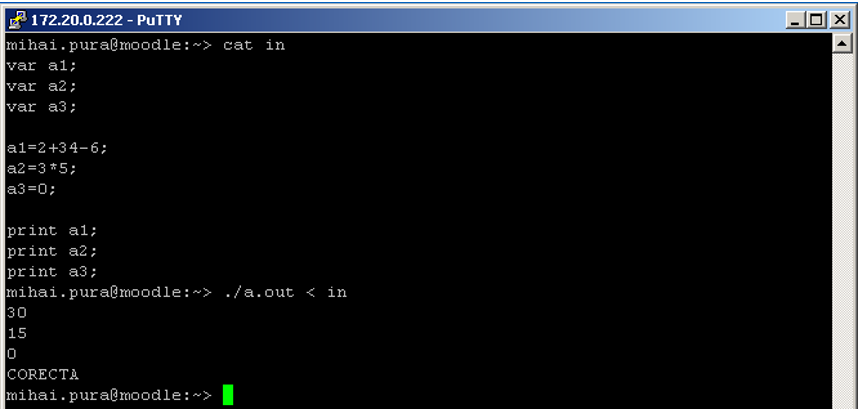
\includegraphics[width=\linewidth]{poza1.png}
\end{figure}
\end{frame}



\begin{frame}
\frametitle{Ex4 din arhiva}
\begin{figure}
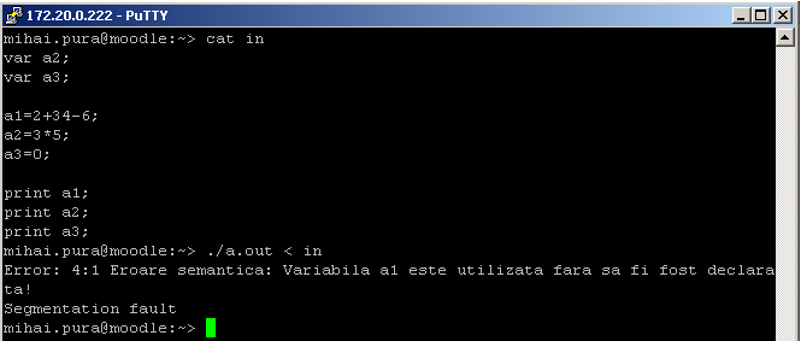
\includegraphics[width=\linewidth]{picture1.png} 
\end{figure}
\end{frame}



\begin{frame}
\frametitle{Ex4 din arhiva}
\begin{figure}
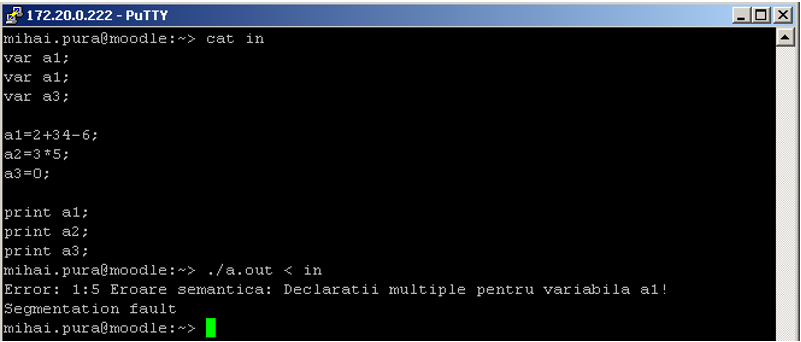
\includegraphics[width=\linewidth]{poza2.png} 
\end{figure}
\end{frame}



\begin{frame}
\frametitle{Ex4 din arhiva}
\begin{figure}
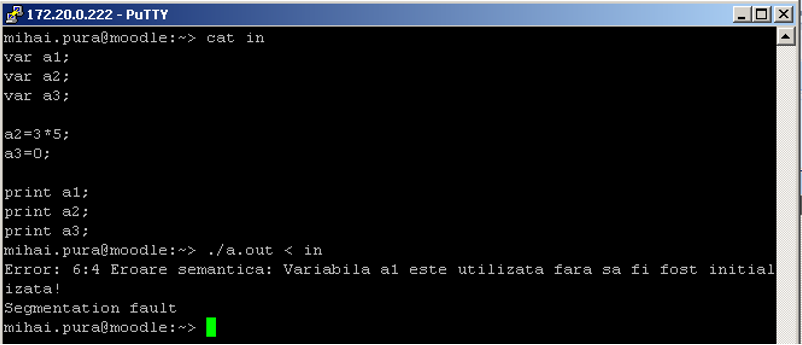
\includegraphics[width=\linewidth]{poza3.png} 
\end{figure}
\end{frame}



\begin{frame}
\frametitle{Ex4 din arhiva}
\begin{figure}
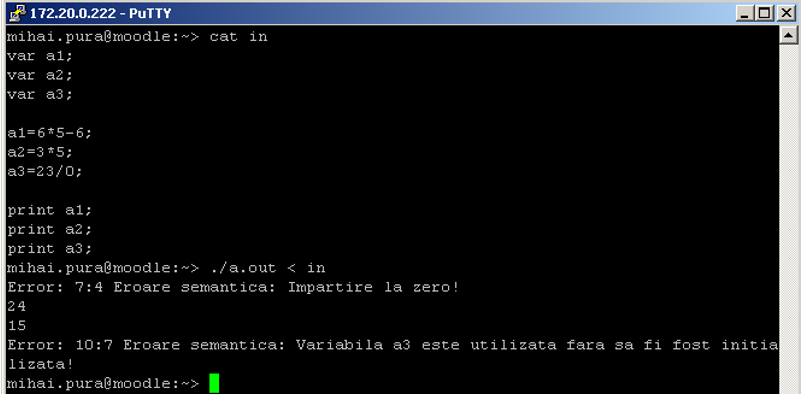
\includegraphics[width=\linewidth]{poza4.png} 
\end{figure}
\end{frame}



\begin{frame}
\frametitle{Arhitectura MIPS}
\begin{itemize}
\item
Procesorul este format din:
\begin{itemize}
\item
O unitate centrala de procesare (CPU) principala;
\item
Doua co-procesoare:
\begin{itemize}
\item
Unul pentru operatiile cu numere reale;
\item
Unul pentru gestiunea memoriei.
\end{itemize}
\end{itemize}
\item
Dimensiunea unui cuvânt este de 32 de biti (numarul de biti pe care un CPU îl poate procesa la un moment dat).
\item
Procesorul are un numar de 32 de registri, fiecare de dimensiunea unui cuvânt, unii cu destinatii speciale, altii pentru utilizarea generala.
\item
Co-procesorul dedicat operatiilor cu numere reale are si el 32 de registrii.
\item
Toate instructiunile sunt codate printr-un singur format, de lungimea unui cuvânt.
\item
Toate operatiile cu date sunt de tip registru la registru.
\item
Referintele la memorie sunt numai de tip load/store.
\end{itemize} 
\end{frame}



\begin{frame}
\frametitle{Cei 32 de registrii MIPS}
\begin{figure}
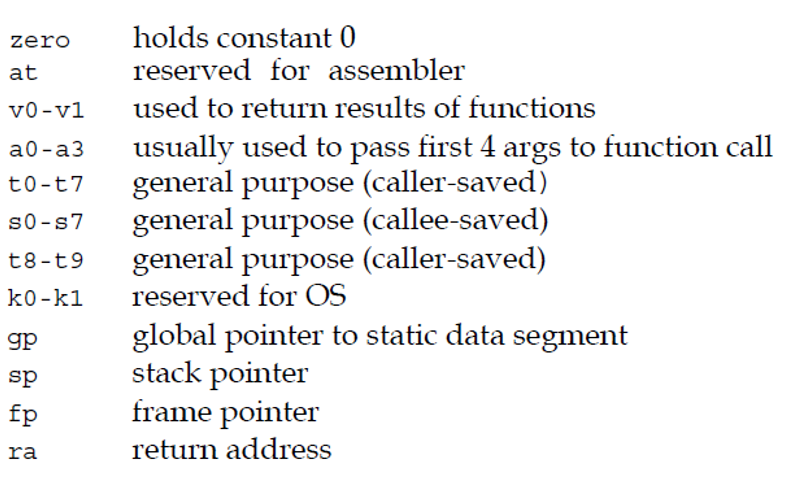
\includegraphics[width=\linewidth]{poza5.png} 
\end{figure}
\end{frame}



\begin{frame}
\frametitle{Modul de adresare}
\begin{itemize}
\item
Masina ofera un singur mod de adresare:
\item \hspace{25mm}
\textcolor{red}{c (rx)}
\item
Accesarea locatiei de la offsetul \textcolor{red}{c} (pozitiv sau negativ), relativ la adresa de memorie stocata în registrul \textcolor{red}{rx}.
\item
Instructiunile load si store opereaza numai asupra datelor aliniate: o cantitate este aliniata numai daca adresa sa este un multiplu al dimensiunii sale în octeti.
\end{itemize}
\end{frame}



\begin{frame}
\frametitle{Formatul spatiului de adrese}
\begin{itemize}
\item
Spatiul de adrese al unui program pe o masina MIPS este format din mai multe segmente:
\item
În partea de jos este \textcolor{red}{segmentul de text} (contine instructiunile programului) – dimensiune fixa, setata la compilare, care nu se poate modifica.
\item
Urmeaza apoi \textcolor{red}{segmentul de date statice} (contine obiectele a caror adresa si dimensiune sunt cunoscute compilatorului si link-editorului în momentul compilarii) – dimensiune fixa, setata la compilare, care nu se poate modifica.
\item
În partea urmatoare se afla \textcolor{red}{segmentul de date dinamice} numit si \textcolor{red}{heap} (dimensiunea sa creste în functie de appelurile de alocare de memorie).
\item
În partea de sus a spatiului de adrese este \textcolor{red}{stiva programului}. Aceasta creste în jos, catre \textcolor{red}{heap}.
\end{itemize}
\end{frame}



\begin{frame}
\frametitle{SPIM}
\begin{itemize}
\item
SPIM este un simulator pentru MIPS32.
\item
Permite citirea si executia de programe scrise în limbaj de asamblare.
\item
Nu ruleaza executabile (programe binare compilate).
\end{itemize}
\end{frame}



\begin{frame}[shrink=20]
\frametitle{Un exemplu de program MIPS}
\begin{itemize}
\item \qquad
	.text
\item \qquad
	.globl main
\item 	
main:
\item \qquad
	li \hspace{10mm} \$t1, 1
\item \qquad
	li \hspace{10mm}	\$t2, 32
\item \qquad
	addu \hspace{4mm} \$t3,\$t1,\$t2
\item \qquad
	la \hspace{9mm}	\$a0, egal
\item \qquad
	li \hspace{10mm}	\$v0, 4
\item \qquad
	syscall
\item \qquad
	move \hspace{3mm} \$a0, \$t3
\item \qquad
	li \hspace{10mm}	\$v0, 1
\item \qquad
	syscall
\item \qquad
	la \hspace{9mm}	\$a0, linie\underline{ }noua
\item \qquad
	li \hspace{10mm}	\$v0, 4
\item \qquad
	syscall
\item \qquad
	li \hspace{10mm}	\$v0, 10
\item \qquad
	syscall
\item \qquad
	.data
\item
egal:	\hspace{11mm}	.asciiz \qquad	"="
\item
linie\underline{ }noua: \hspace{2mm} .asciiz \qquad	"\textbackslash{n}"
\end{itemize}
\end{frame}



\begin{frame}
\frametitle{Un exemplu de program MIPS}
\begin{figure}
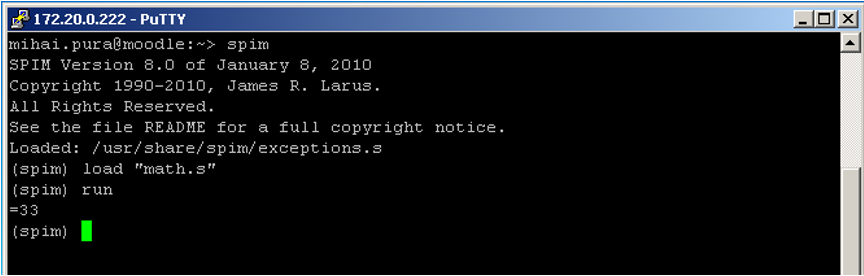
\includegraphics[width=\linewidth]{poza6.png} 
\end{figure}
\end{frame}



\begin{frame}[shrink=10]
\frametitle{Ex5 din arhiva - Generarea codului pentru limbajul expresiilor aritmetice}
\begin{itemize}
\item
\%\{
\item \quad
	\#include "y.tab.h"
\item \quad
	extern int yylval;
\item \quad
	int lineNo = 1; 
\item \quad
     int colNo = 1;
\item
\%\}
\item
\%\%
\item
"+" \qquad	\{ colNo++; return TOK\underline{ }PLUS; \}
\item
"-"	\qquad \hspace{0.8mm}	\{ colNo++; return TOK\underline{ }MINUS; \}
\item
"*"	\qquad \hspace{0.3mm}	\{ colNo++; return TOK\underline{ }MULTIPLY; \}
\item
"/"	\qquad \hspace{0.3mm}	\{ colNo++; return TOK\underline{ }DIVIDE; \}
\item
"("	\qquad \hspace{0.5mm}	\{ colNo++; return TOK\underline{ }LEFT; \}
\item
")"	\qquad \hspace{0.5mm}	\{ colNo++; return TOK\underline{ }RIGHT; \}
\item
";"	\qquad \hspace{1mm}	\{ colNo++; return ';'; \}
\item
0|[1-9][0-9]* \qquad	\{ colNo+=strlen(yytext); yylloc.first\underline{ }line = lineNo; yylloc.first\underline{ }column = colNo; yylval = atoi(yytext); return TOK\underline{ }NUMBER; \}
.		\{ colNo++; return TOK\underline{ }ERROR; \}
\item
\textbackslash{n} \hspace{2mm}	\qquad	\{ lineNo++;colNo=1; \}
\item
\%\%
\end{itemize}
\end{frame}



\begin{frame}[shrink=10]
\frametitle{Ex5 din arhiva}
\begin{itemize}
\item
\%\{
\item \qquad \vspace{5mm}
	\#include <stdio.h>
\item \qquad \vspace{5mm}
	FILE * yyies = NULL;
\item \qquad
          int EsteCorecta = 1;
\item \qquad \vspace{5mm}
	char msg[50];
\item \qquad 
	int Prima = 0;
\item
\%\}
\item \vspace{5mm}
\%token TOK\underline{ }PLUS TOK\underline{ }MINUS TOK\underline{ }MULTIPLY TOK\underline{ }DIVIDE TOK\underline{ }LEFT TOK\underline{ }RIGHT
\item
\%token TOK\underline{ }NUMBER TOK\underline{ }ERROR
\item \vspace{5mm}
\%start S
\item \vspace{5mm}
\%left TOK\underline{ }PLUS TOK\underline{ }MINUS
\item
\%left TOK\underline{ }MULTIPLY TOK\underline{ }DIVIDE
\end{itemize}
\end{frame}



\begin{frame}
\frametitle{Ex5 din arhiva}
\begin{itemize}
\item
\%\%
\item
S : 
\item \quad
    |
\item \quad
    E ';' S 
\item \qquad
	\{ 
\item \qquad \hspace{4mm}
		fprintf(yyies,"\textbackslash{t}la\textbackslash{t}\$a0, egal\textbackslash{n}\textbackslash{t}li\textbackslash{t}\$v0, 4\textbackslash{n}\textbackslash{t}syscall\textbackslash{n}\textbackslash{t}move\textbackslash{t}\$a0, \$t1\textbackslash{n}\textbackslash{t}li\textbackslash{t}\$v0, 1\textbackslash{n}\textbackslash{t}syscall\textbackslash{n}");
\item \qquad \hspace{4mm}
		fprintf(yyies, "\textbackslash{t}la\textbackslash{t}\$a0, linie\underline{ }noua\textbackslash{n}\textbackslash{t}li\textbackslash{t}\$v0, 4\textbackslash{n}\textbackslash{t}syscall\textbackslash{n}"); 
\item \qquad \hspace{4mm}
		Prima = 0;
\item \qquad
	\}
\item \quad
    | 
\item \quad
    error ';' S
\item \qquad
       \{ EsteCorecta = 0; \}
\item \quad
    ;
\end{itemize}
\end{frame}



\begin{frame}
\frametitle{Ex5 din arhiva}
\begin{itemize}
\item
E : E TOK\underline{ }PLUS E 
\item \quad \hspace{2mm}
	\{ 
\item \qquad \hspace{2mm}
		fprintf(yyies, "\textbackslash{t}add\textbackslash{t}\$t1,\$t1,\$t2\textbackslash{n}");
\item \qquad \hspace{2mm}
		Prima = 1;
\item \quad \hspace{2mm}
	\}
\item \quad
    |
\item \quad    
    E TOK\underline{ }MINUS E
\item \quad \hspace{2mm}
	\{
\item \qquad \hspace{2mm}
		fprintf(yyies, "\textbackslash{t}sub\textbackslash{t}\$t1,\$t1,\$t2\textbackslash{n}");
\item \qquad \hspace{2mm}
		Prima = 1;
\item \quad \hspace{2mm}
	\}
\item \quad
    |
\end{itemize}
\end{frame}



\begin{frame}
\frametitle{Ex5 din arhiva}
\begin{itemize}
\item
 E TOK\underline{ }MULTIPLY E 
\item \quad
	\{
\item \qquad 
		if(Prima == 2)
\item \qquad 
		\{
\item \qquad \quad
			fprintf(yyies, "\textbackslash{t}mult\textbackslash{t}\$t1,\$t2\textbackslash{n}");
\item \qquad \quad
			fprintf(yyies, "\textbackslash{t}mflo\textbackslash{t}\$t1\textbackslash{n}");
\item \qquad
		\}
\item \qquad
		else 
\item \qquad
		\{
\item \qquad \quad
			fprintf(yyies, "\textbackslash{t}mult\textbackslash{t}\$t2,\$t3\textbackslash{n}");
\item \qquad \quad
			fprintf(yyies, "\textbackslash{t}mflo\textbackslash{t}\$t2\textbackslash{n}");
\item \qquad 
		\}
\item \qquad
		Prima = 1;
\item \quad
	\}
\item \vspace{5mm}
    |
\end{itemize}
\end{frame}



\begin{frame}[shrink=20]
\frametitle{Ex5 din arhiva}
\begin{itemize}
\item
E TOK\underline{ }DIVIDE E 
\item \quad
	\{ 
\item \quad \hspace{2mm}
	  if(\$3 == 0) 
\item \quad \hspace{2mm}
	  \{ 
\item \qquad \hspace{2mm}
	      sprintf(msg,"\%d:\%d Eroare semantica: Impartire la zero!", @1.first\underline{ }line, @1.first\underline{ }column);
\item \qquad \hspace{2mm}
	      yyerror(msg);
\item \qquad \hspace{2mm}
	      YYERROR;
\item \quad \hspace{2mm}
	  \} 
\item \quad \hspace{2mm}
	  else
\item \quad \hspace{2mm}
	  \{
\item \qquad \hspace{8mm}
		if(Prima == 2)
\item \qquad \hspace{8mm}
		\{
\item \qquad \hspace{12mm}
			fprintf(yyies, "\textbackslash{t}div\textbackslash{t}\$t1,\$t2\textbackslash{n}");
\item \qquad \hspace{12mm}
			fprintf(yyies, "\textbackslash{t}mflo\textbackslash{t}\$t1\textbackslash{n}");
\item \qquad \hspace{8mm}
		\}
\item \qquad \hspace{8mm}
		else
\item \qquad \hspace{8mm}
		\{
\item \qquad \hspace{12mm}
			fprintf(yyies, "\textbackslash{t}div\textbackslash{t}\$t2,\$t3\textbackslash{n}");
\item \qquad \hspace{12mm}
			fprintf(yyies, "\textbackslash{t}mflo\textbackslash{t}\$t2\textbackslash{n}");
\item \qquad \hspace{8mm}
		\}
\item \qquad \hspace{8mm}
		Prima = 1;
\item \qquad \hspace{2mm}
	  \}
\item \quad \hspace{2mm}
	\}
\item \quad
    | 
\end{itemize}
\end{frame}



\begin{frame}[shrink=10]
\frametitle{Ex5 din arhiva}
\begin{itemize}
\item
 TOK\underline{ }NUMBER 
\item \quad
	\{ 
\item \qquad
		if(Prima == 0)
\item \qquad
		\{
\item \qquad \quad
			fprintf(yyies, "\textbackslash{t}li\textbackslash{t}\$t1, \%d\textbackslash{n}", \$1); 
\item \qquad \quad		
			Prima = 1;
\item \qquad
		\}
\item \qquad
		else if(Prima == 1)
\item \qquad
		\{
\item \qquad \quad
			fprintf(yyies, "\textbackslash{t}li\textbackslash{t}\$t2, \%d\textbackslash{n}", \$1);
\item \qquad \quad
			Prima = 2;
\item \qquad
		\}
\item \qquad
		else
\item \qquad
		\{
\item \qquad \quad
			fprintf(yyies, "\textbackslash{t}li\textbackslash{t}\$t3, \%d\textbackslash{n}", \$1); 
\item \qquad \quad
			Prima = 3;
\item \qquad
		\}
\item \quad
	\}
\item \hspace{2mm}
    ;
\item
\%\%
\end{itemize}
\end{frame}



\begin{frame}[shrink=10]
\frametitle{Ex5 din arhiva}
\begin{itemize}
\item
int main()
\item
\{
\item \quad
	yyies = fopen("math.s","w");
\item \quad \vspace{5mm}
	fprintf(yyies, "\textbackslash{t}.text\textbackslash{n}\textbackslash{t}.globl main\textbackslash{n}main:\textbackslash{n}");
\item \quad \vspace{5mm}
	yyparse();
\item \quad 
		fprintf(yyies,"\textbackslash{t}li\textbackslash{t}\$v0, 10\textbackslash{n}\textbackslash{t}syscall\textbackslash{n}\textbackslash{t}.data\textbackslash{n}egal:\textbackslash{t}\textbackslash{t}.asciiz  \text{\textbackslash "}"\textbackslash{n}linie\underline{ }noua:\textbackslash{t}.asciiz\textbackslash{t}\text{\textbackslash "}\text{\textbackslash}\textbackslash{n}\text{\textbackslash "}");
\item \quad \vspace{5mm}
	fclose(yyies);
\item \quad 
	if(EsteCorecta == 1)
\item \quad 
	\{
\item \qquad 
		printf("CORECTA\textbackslash{n}");		
\item \quad	\vspace{5mm}
	\}	
\item \qquad 
       return 0;
\item
\}
\end{itemize}
\end{frame}



\begin{frame}
\frametitle{Ex5 din arhiva}
\begin{itemize}
\item
int yyerror(const char *msg)
\item
\{
\item \quad
	printf("Error: \%s\textbackslash{n}", msg);
\item \quad
	return 1;
\item
\}
\end{itemize}
\end{frame}



\begin{frame}[shrink=10]
\frametitle{Ex5 din arhiva}
\begin{itemize}
\item
Ex: 2*3+4+2*2-1-5+2+3*2-4/2+3;
\item \vspace{5mm}
	.text
\item \quad
	.globl main
\item
main:
\item \quad
	li \hspace{10mm} \$t1, 2
\item \quad
	li \hspace{10mm} \$t2, 3
\item \quad
	mult \hspace{4.5mm} \$t1,\$t2
\item \quad
	mflo \hspace{4.7mm} \$t1
\item \quad \vspace{5mm}
	li \hspace{10mm} \$t2, 4
\item \quad
	add \hspace{6mm} \$t1,\$t1,\$t2
\item \quad \vspace{5mm}
	li \hspace{10mm} \$t2, 2
\item \quad
	li \hspace{10mm} \$t3, 2
\item \quad
	mult \hspace{4.5mm} \$t2,\$t3
\item \quad
	mflo \hspace{4.7mm} \$t2
\end{itemize}
\end{frame}



\begin{frame}[shrink=20]
\frametitle{Ex5 din arhiva}
\begin{itemize}
\item \vspace{5mm}
Ex: 2*3+4+2*2-1-5+2+3*2-4/2+3;
\item \quad \vspace{5mm}
	add \hspace{6mm} \$t1,\$t1,\$t2
\item \quad 
	li \hspace{10mm} \$t2, 1
\item \quad \vspace{5mm}
	sub \hspace{6.5mm} \$t1,\$t1,\$t2
\item \quad 
	li \hspace{10mm} \$t2, 5
\item \quad \vspace{5mm}
	sub \hspace{6.5mm} \$t1,\$t1,\$t2
\item \quad 
	li \hspace{10mm} \$t2, 2
\item \quad \vspace{5mm}
	add \hspace{6mm} \$t1,\$t1,\$t2
\item \quad 
	li \hspace{10mm} \$t2, 3
\item \quad
	li \hspace{10mm} \$t3, 2
\item \quad
	mult \hspace{4.5mm} \$t2,\$t3
\item \quad \vspace{5mm}
	mflo \hspace{4.8mm}  \$t2
\item \quad 
	add	\hspace{6mm} \$t1,\$t1,\$t2
\end{itemize}
\end{frame}



\begin{frame}
\frametitle{Ex5 din arhiva}
\begin{itemize}
\item  
Ex: 2*3+4+2*2-1-5+2+3*2-4/2+3;
\item \quad
	li \hspace{10mm} \$t2, 4
\item \quad
	li \hspace{10mm} \$t3, 2
\item \quad
	div \hspace{8.5mm}\$t2,\$t3
\item \quad \vspace{5mm}
	mflo \hspace{4.7mm} \$t2
\item \quad \vspace{5mm}
	sub \hspace{6.5mm} \$t1,\$t1,\$t2
\item \quad 
	li \hspace{10mm} \$t2, 3
\item \quad
	add \hspace{6mm} \$t1,\$t1,\$t2
\end{itemize}
\end{frame}



\begin{frame}[shrink=20]
\frametitle{Ex5 din arhiva}
\begin{itemize}
\item  \quad
    la \hspace{13.2mm}	\$a0, egal
\item  \quad
	li \hspace{14mm}	\$v0, 4
\item  \quad \vspace{5mm}
	syscall
\item  \quad 
	move \hspace{7.5mm} \$a0, \$t1
\item \quad
	li \hspace{14mm} \$v0, 1
\item \quad \vspace{5mm}
	syscall
\item \quad
	la \hspace{13.2mm} \$a0, linie\underline{ }noua
\item \quad
	li \hspace{14mm} \$v0, 4
\item \quad \vspace{5mm}
	syscall
\item \quad
	li \hspace{14mm} \$v0, 10
\item \quad \vspace{5mm}
	syscall
\item \quad
	.data
\item 
egal: \hspace{11mm} .asciiz	"="
\item 
linie\underline{ }noua: \hspace{2mm}	.asciiz	"\textbackslash{n}"
\end{itemize}
\end{frame}



\begin{frame}
\frametitle{Ex5 din arhiva}
\begin{figure}
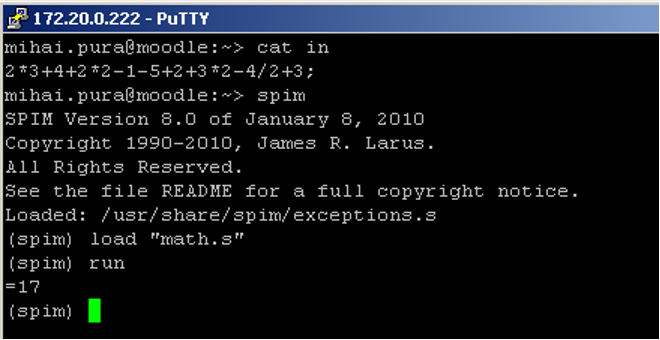
\includegraphics[width=\linewidth]{poza7.png} 
\end{figure}
\end{frame}



\begin{frame}
\frametitle{Generarea codului pentru limbajul expresiilor aritmetice}
\begin{center}
\begin{tabular}{cc|c|} \cline{1-2}
\multicolumn{1}{|c|}{\textcolor{red}{Intrare}} & {2*3+4+2*2-1-5+2+3*2-4/2+3} \\ \cline{1-2}
\multicolumn{1}{|c|}{\textcolor{red}{Look ahead}} & $\varepsilon$ \\ \cline{1-2}
\multicolumn{1}{|c|}{\textcolor{red}{Stiva}}  \\
\cline{1-1} \cline{3-3}
\multicolumn{1}{|c|}{$\varepsilon$} & & \textit{\quad}\\
\cline{1-1} \cline{3-3}
\end{tabular}
\end{center}
\end{frame}



\begin{frame}
\frametitle{Generarea codului pentru limbajul expresiilor aritmetice}
\begin{center}
\begin{tabular}{cc|c|} \cline{1-2}
\multicolumn{1}{|c|}{\textcolor{red}{Intrare}} & {2*3+4+2*2-1-5+2+3*2-4/2+3} \\ \cline{1-2}
\multicolumn{1}{|c|}{\textcolor{red}{Look ahead}} & NR \\ \cline{1-2}
\multicolumn{1}{|c|}{\textcolor{red}{Stiva}}  \\
\cline{1-1} \cline{3-3}
\multicolumn{1}{|c|}{$\varepsilon$} & & \textit{\quad}\\
\cline{1-1} \cline{3-3}
\end{tabular}
\end{center}
\end{frame}



\begin{frame}
\frametitle{Generarea codului pentru limbajul expresiilor aritmetice}
\begin{center}
\begin{tabular}{cc|c|} \cline{1-2}
\multicolumn{1}{|c|}{\textcolor{red}{Intrare}} & {2*3+4+2*2-1-5+2+3*2-4/2+3} \\ \cline{1-2}
\multicolumn{1}{|c|}{\textcolor{red}{Look ahead}} & * \\ \cline{1-2}
\multicolumn{1}{|c|}{\textcolor{red}{Stiva}}  \\
\cline{1-1} \cline{3-3}
\multicolumn{1}{|c|}{NR} & & \textit{\quad}\\
\cline{1-1} \cline{3-3}
\end{tabular}
\end{center}
\end{frame}



\begin{frame}
\frametitle{Generarea codului pentru limbajul expresiilor aritmetice}
\begin{center}
\begin{tabular}{cc|c|} \cline{1-2}
\multicolumn{1}{|c|}{\textcolor{red}{Intrare}} & {2*3+4+2*2-1-5+2+3*2-4/2+3} \\ \cline{1-2}
\multicolumn{1}{|c|}{\textcolor{red}{Look ahead}} & * \\ \cline{1-2}
\multicolumn{1}{|c|}{\textcolor{red}{Stiva}}  \\
\cline{1-1} \cline{3-3}
\multicolumn{1}{|c|}{E} & & {li \quad \$t1, 2}\\
\cline{1-1} \cline{3-3}
\end{tabular}
\end{center}
\end{frame}



\begin{frame}
\frametitle{Generarea codului pentru limbajul expresiilor aritmetice}
\begin{center}
\begin{tabular}{cc|c|} \cline{1-2}
\multicolumn{1}{|c|}{\textcolor{red}{Intrare}} & {2*3+4+2*2-1-5+2+3*2-4/2+3} \\ \cline{1-2}
\multicolumn{1}{|c|}{\textcolor{red}{Look ahead}} & NR \\ \cline{1-2}
\multicolumn{1}{|c|}{\textcolor{red}{Stiva}}  \\
\cline{1-1} \cline{3-3}
\multicolumn{1}{|c|}{*} & & {}\\
\cline{1-1} \cline{3-3} 
\multicolumn{1}{|c|}{E} & & {li \quad \$t1, 2}\\
\cline{1-1} \cline{3-3}
\end{tabular}
\end{center}
\end{frame}



\begin{frame}
\frametitle{Generarea codului pentru limbajul expresiilor aritmetice}
\begin{center}
\begin{tabular}{cc|c|} \cline{1-2}
\multicolumn{1}{|c|}{\textcolor{red}{Intrare}} & {2*3+4+2*2-1-5+2+3*2-4/2+3} \\ \cline{1-2}
\multicolumn{1}{|c|}{\textcolor{red}{Look ahead}} & + \\ \cline{1-2}
\multicolumn{1}{|c|}{\textcolor{red}{Stiva}}  \\
\cline{1-1} \cline{3-3}
\multicolumn{1}{|c|}{NR} & & {}\\
\cline{1-1} \cline{3-3} 
\multicolumn{1}{|c|}{*} & & {}\\
\cline{1-1} \cline{3-3}
\multicolumn{1}{|c|}{E} & & {li \quad \$t1, 2}\\
\cline{1-1} \cline{3-3}
\end{tabular}
\end{center}
\end{frame}



\begin{frame}
\frametitle{Generarea codului pentru limbajul expresiilor aritmetice}
\begin{center}
\begin{tabular}{cc|c|} \cline{1-2}
\multicolumn{1}{|c|}{\textcolor{red}{Intrare}} & {2*3+4+2*2-1-5+2+3*2-4/2+3} \\ \cline{1-2}
\multicolumn{1}{|c|}{\textcolor{red}{Look ahead}} & + \\ \cline{1-2}
\multicolumn{1}{|c|}{\textcolor{red}{Stiva}}  \\
\cline{1-1} \cline{3-3}
\multicolumn{1}{|c|}{E} & & {li \quad \$t2, 3}\\
\cline{1-1} \cline{3-3} 
\multicolumn{1}{|c|}{*} & & {}\\
\cline{1-1} \cline{3-3}
\multicolumn{1}{|c|}{E} & & {li \quad \$t1, 2}\\
\cline{1-1} \cline{3-3}
\end{tabular}
\end{center}
\end{frame}



\begin{frame}
\frametitle{Generarea codului pentru limbajul expresiilor aritmetice}
\begin{center}
\begin{tabular}{cc|c|} \cline{1-2}
\multicolumn{1}{|c|}{\textcolor{red}{Intrare}} & {2*3+4+2*2-1-5+2+3*2-4/2+3} \\ \cline{1-2}
\multicolumn{1}{|c|}{\textcolor{red}{Look ahead}} & + \\ \cline{1-2}
\multicolumn{1}{|c|}{\textcolor{red}{Stiva}}  \\
\cline{1-1} \cline{3-3}
\multicolumn{1}{|c|}{\multirow{2}{*}{E}} & & {mult\quad \$t1,\$t2 }\\
\multicolumn{1}{|c|}{} & & {mflo \quad \$t1} \\
\cline{1-1} \cline{3-3} 
\end{tabular}
\end{center}
\end{frame}



\begin{frame}
\frametitle{Generarea codului pentru limbajul expresiilor aritmetice}
\begin{center}
\begin{tabular}{cc|c|} \cline{1-2}
\multicolumn{1}{|c|}{\textcolor{red}{Intrare}} & {2*3+4+2*2-1-5+2+3*2-4/2+3} \\ \cline{1-2}
\multicolumn{1}{|c|}{\textcolor{red}{Look ahead}} & NR \\ \cline{1-2}
\multicolumn{1}{|c|}{\textcolor{red}{Stiva}}  \\
\cline{1-1} \cline{3-3}
\multicolumn{1}{|c|}{+} & & {}\\
\cline{1-1} \cline{3-3}
\multicolumn{1}{|c|}{\multirow{2}{*}{E}} & & { mult\quad \$t1,\$t2 }\\
\multicolumn{1}{|c|}{} & & { mflo \quad \$t1} \\
\cline{1-1} \cline{3-3} 
\end{tabular}
\end{center}
\end{frame}



\begin{frame}
\frametitle{Generarea codului pentru limbajul expresiilor aritmetice}
\begin{center}
\begin{tabular}{cc|c|} \cline{1-2}
\multicolumn{1}{|c|}{\textcolor{red}{Intrare}} & {2*3+4+2*2-1-5+2+3*2-4/2+3} \\ \cline{1-2}
\multicolumn{1}{|c|}{\textcolor{red}{Look ahead}} & + \\ \cline{1-2}
\multicolumn{1}{|c|}{\textcolor{red}{Stiva}}  \\
\cline{1-1} \cline{3-3}
\multicolumn{1}{|c|}{NR} & & {}\\
\cline{1-1} \cline{3-3}
\multicolumn{1}{|c|}{+} & & {}\\
\cline{1-1} \cline{3-3}
\multicolumn{1}{|c|}{\multirow{2}{*}{E}} & & { mult\quad \$t1,\$t2 }\\
\multicolumn{1}{|c|}{} & & { mflo \quad \$t1} \\
\cline{1-1} \cline{3-3} 
\end{tabular}
\end{center}
\end{frame}



\begin{frame}
\frametitle{Generarea codului pentru limbajul expresiilor aritmetice}
\begin{center}
\begin{tabular}{cc|c|} \cline{1-2}
\multicolumn{1}{|c|}{\textcolor{red}{Intrare}} & {2*3+4+2*2-1-5+2+3*2-4/2+3} \\ \cline{1-2}
\multicolumn{1}{|c|}{\textcolor{red}{Look ahead}} & + \\ \cline{1-2}
\multicolumn{1}{|c|}{\textcolor{red}{Stiva}}  \\
\cline{1-1} \cline{3-3}
\multicolumn{1}{|c|}{E} & & {li \quad \$t2, 4}\\
\cline{1-1} \cline{3-3}
\multicolumn{1}{|c|}{+} & & {}\\
\cline{1-1} \cline{3-3}
\multicolumn{1}{|c|}{\multirow{2}{*}{E}} & & { mult\quad \$t1,\$t2 }\\
\multicolumn{1}{|c|}{} & & { mflo \quad \$t1} \\
\cline{1-1} \cline{3-3} 
\end{tabular}
\end{center}
\end{frame}



\begin{frame}
\frametitle{Generarea codului pentru limbajul expresiilor aritmetice}
\begin{center}
\begin{tabular}{cc|c|} \cline{1-2}
\multicolumn{1}{|c|}{\textcolor{red}{Intrare}} & {2*3+4+2*2-1-5+2+3*2-4/2+3} \\ \cline{1-2}
\multicolumn{1}{|c|}{\textcolor{red}{Look ahead}} & + \\ \cline{1-2}
\multicolumn{1}{|c|}{\textcolor{red}{Stiva}}  \\
\cline{1-1} \cline{3-3}
\multicolumn{1}{|c|}{E} & & {add \quad \$t1,\$t1,\$t2}\\
\cline{1-1} \cline{3-3}
\end{tabular}
\end{center}
\end{frame}



\begin{frame}
\frametitle{Generarea codului pentru limbajul expresiilor aritmetice}
\begin{center}
\begin{tabular}{cc|c|} \cline{1-2}
\multicolumn{1}{|c|}{\textcolor{red}{Intrare}} & {2*3+4+2*2-1-5+2+3*2-4/2+3} \\ \cline{1-2}
\multicolumn{1}{|c|}{\textcolor{red}{Look ahead}} & + \\ \cline{1-2}
\multicolumn{1}{|c|}{\textcolor{red}{Stiva}}  \\
\cline{1-1} \cline{3-3}
\multicolumn{1}{|c|}{+} & & {}\\
\cline{1-1} \cline{3-3}
\multicolumn{1}{|c|}{E} & & {add \quad \$t1,\$t1,\$t2}\\
\cline{1-1} \cline{3-3}
\end{tabular}
\end{center}
\end{frame}



\begin{frame}
\frametitle{Generarea codului pentru limbajul expresiilor aritmetice}
\begin{center}
\begin{tabular}{cc|c|} \cline{1-2}
\multicolumn{1}{|c|}{\textcolor{red}{Intrare}} & {2*3+4+2*2-1-5+2+3*2-4/2+3} \\ \cline{1-2}
\multicolumn{1}{|c|}{\textcolor{red}{Look ahead}} & + \\ \cline{1-2}
\multicolumn{1}{|c|}{\textcolor{red}{Stiva}}  \\
\cline{1-1} \cline{3-3}
\multicolumn{1}{|c|}{E} & & {li \quad \$t2, 2}\\
\cline{1-1} \cline{3-3}
\multicolumn{1}{|c|}{+} & & {}\\
\cline{1-1} \cline{3-3}
\multicolumn{1}{|c|}{E} & & {add \quad \$t1,\$t1,\$t2}\\
\cline{1-1} \cline{3-3}
\end{tabular}
\end{center}
\end{frame}



\begin{frame}
\frametitle{Generarea codului pentru limbajul expresiilor aritmetice}
\begin{center}
\begin{tabular}{cc|c|} \cline{1-2}
\multicolumn{1}{|c|}{\textcolor{red}{Intrare}} & {2*3+4+2*2-1-5+2+3*2-4/2+3} \\ \cline{1-2}
\multicolumn{1}{|c|}{\textcolor{red}{Look ahead}} & + \\ \cline{1-2}
\multicolumn{1}{|c|}{\textcolor{red}{Stiva}}  \\
\cline{1-1} \cline{3-3}
\multicolumn{1}{|c|}{*} & & {}\\
\cline{1-1} \cline{3-3}
\multicolumn{1}{|c|}{E} & & {li \quad \$t2, 2}\\
\cline{1-1} \cline{3-3}
\multicolumn{1}{|c|}{+} & & {}\\
\cline{1-1} \cline{3-3}
\multicolumn{1}{|c|}{E} & & {add \quad \$t1,\$t1,\$t2}\\
\cline{1-1} \cline{3-3}
\end{tabular}
\end{center}
\end{frame}



\begin{frame}
\frametitle{Generarea codului pentru limbajul expresiilor aritmetice}
\begin{center}
\begin{tabular}{cc|c|} \cline{1-2}
\multicolumn{1}{|c|}{\textcolor{red}{Intrare}} & {2*3+4+2*2-1-5+2+3*2-4/2+3} \\ \cline{1-2}
\multicolumn{1}{|c|}{\textcolor{red}{Look ahead}} & + \\ \cline{1-2}
\multicolumn{1}{|c|}{\textcolor{red}{Stiva}}  \\
\cline{1-1} \cline{3-3}
\multicolumn{1}{|c|}{NR} & & {}\\
\cline{1-1} \cline{3-3}
\multicolumn{1}{|c|}{*} & & {}\\
\cline{1-1} \cline{3-3}
\multicolumn{1}{|c|}{E} & & {li \quad \$t2, 2}\\
\cline{1-1} \cline{3-3}
\multicolumn{1}{|c|}{+} & & {}\\
\cline{1-1} \cline{3-3}
\multicolumn{1}{|c|}{E} & & {add \quad \$t1,\$t1,\$t2}\\
\cline{1-1} \cline{3-3}
\end{tabular}
\end{center}
\end{frame}



\begin{frame}
\frametitle{Generarea codului pentru limbajul expresiilor aritmetice}
\begin{center}
\begin{tabular}{cc|c|} \cline{1-2}
\multicolumn{1}{|c|}{\textcolor{red}{Intrare}} & {2*3+4+2*2-1-5+2+3*2-4/2+3} \\ \cline{1-2}
\multicolumn{1}{|c|}{\textcolor{red}{Look ahead}} & + \\ \cline{1-2}
\multicolumn{1}{|c|}{\textcolor{red}{Stiva}}  \\
\cline{1-1} \cline{3-3}
\multicolumn{1}{|c|}{E} & & {li \quad \$t3, 2}\\
\cline{1-1} \cline{3-3}
\multicolumn{1}{|c|}{*} & & {}\\
\cline{1-1} \cline{3-3}
\multicolumn{1}{|c|}{E} & & {li \quad \$t2, 2}\\
\cline{1-1} \cline{3-3}
\multicolumn{1}{|c|}{+} & & {}\\
\cline{1-1} \cline{3-3}
\multicolumn{1}{|c|}{E} & & {add \quad \$t1,\$t1,\$t2}\\
\cline{1-1} \cline{3-3}
\end{tabular}
\end{center}
\end{frame}



\begin{frame}
\frametitle{Generarea codului pentru limbajul expresiilor aritmetice}
\begin{center}
\begin{tabular}{cc|c|} \cline{1-2}
\multicolumn{1}{|c|}{\textcolor{red}{Intrare}} & {2*3+4+2*2-1-5+2+3*2-4/2+3} \\ \cline{1-2}
\multicolumn{1}{|c|}{\textcolor{red}{Look ahead}} & + \\ \cline{1-2}
\multicolumn{1}{|c|}{\textcolor{red}{Stiva}}  \\
\cline{1-1} \cline{3-3}
\multicolumn{1}{|c|}{\multirow{2}{*}{E}} & & { mult\quad \$t2,\$t3 }\\
\multicolumn{1}{|c|}{} & & { mflo \quad \$t2} \\
\cline{1-1} \cline{3-3} 
\multicolumn{1}{|c|}{+} & & {}\\
\cline{1-1} \cline{3-3}
\multicolumn{1}{|c|}{E} & & {add \quad \$t1,\$t1,\$t2}\\
\cline{1-1} \cline{3-3}
\end{tabular}
\end{center}
\end{frame}



\begin{frame}
\frametitle{Generarea codului pentru limbajul expresiilor aritmetice}
\begin{center}
\begin{tabular}{cc|c|} \cline{1-2}
\multicolumn{1}{|c|}{\textcolor{red}{Intrare}} & {2*3+4+2*2-1-5+2+3*2-4/2+3} \\ \cline{1-2}
\multicolumn{1}{|c|}{\textcolor{red}{Look ahead}} & + \\ \cline{1-2}
\multicolumn{1}{|c|}{\textcolor{red}{Stiva}}  \\
\cline{1-1} \cline{3-3}
\multicolumn{1}{|c|}{E} & & {add \quad \$t1,\$t1,\$t2}\\
\cline{1-1} \cline{3-3}
\end{tabular}
\end{center}

\vspace{8mm} \hspace{80mm} s.a.m.d.
\end{frame}



\begin{frame}
\frametitle{flex \& bison - Întrebări recapitulative}
\begin{itemize}
\item
Explicați utilitatea atomului lexical predefinit \textit{error} în funcționarea unui instrument de analiza gramaticală generat cu bison.
\newline

\item
Fie un automat finit epsilon AF. Arătați care dintre flex și bison este cel mai ușor de folosit pentru a implementa un program care să verifice dacă o propoziție p dată aparține lui L(AF) și explicați.
\newline

\item
Arătați de ce informații are nevoie bison/yacc pentru atomii lexicali, pentru a putea efectua analiza semantică.
\end{itemize}
\end{frame}



\begin{frame}{Bibliografie}
\begin{itemize}
\item
Bert Hubert, \textbf{Lex and YACC primer/HOWTO}

\url{http://tldp.org/HOWTO/Lex-YACC-HOWTO.html}
\newline

\item
Tom Niemann, \textbf{Lex \& Yacc}

\url{http://epaperpress.com/lexandyacc/}
\newline

\item
Anthony A. Aaby, \textbf{Compiler Construction using Flex and Bison}

\url{http://foja.dcs.fmph.uniba.sk/kompilatory/docs/compiler.pdf}
\newline

\end{itemize}
\end{frame}



\begin{frame}[shrink=-10]{Bibliografie}
\begin{itemize}
\item
\textbf{Programmed Introduction to MIPS Assembly Language}

\url{http://programmedlessons.org/AssemblyTutorial/index.html}
\newline

\item
\textbf{MIPS Instruction Reference}

\url{http://www.mrc.uidaho.edu/mrc/people/jff/digital/MIPSir.html}
\newline

\end{itemize}
\end{frame}



\end{document}